%% This is file `elsarticle-template-1-num.tex',
%%
%% Copyright 2009 Elsevier Ltd
%%
%% This file is part of the 'Elsarticle Bundle'.
%% ---------------------------------------------
%%
%% It may be distributed under the conditions of the LaTeX Project Public
%% License, either version 1.2 of this license or (at your option) any
%% later version.  The latest version of this license is in
%%    http://www.latex-project.org/lppl.txt
%% and version 1.2 or later is part of all distributions of LaTeX
%% version 1999/12/01 or later.
%%
%% The list of all files belonging to the 'Elsarticle Bundle' is
%% given in the file `manifest.txt'.
%%
%% Template article for Elsevier's document class `elsarticle'
%% with numbered style bibliographic references
%%
%% $Id: elsarticle-template-1-num.tex 149 2009-10-08 05:01:15Z rishi $
%% $URL: http://lenova.river-valley.com/svn/elsbst/trunk/elsarticle-template-1-num.tex $
%%

\documentclass[preprint,authoryear,review,12pt]{elsarticle}
%\documentclass[final,5p,times,twocolumn]{elsarticle}

%% Use the option review to obtain double line spacing
%% \documentclass[preprint,review,12pt]{elsarticle}

%% Use the options 1p,two column; 3p; 3p,twocolumn; 5p; or 5p,twocolumn
%% for a journal layout:
%% \documentclass[final,1p,times]{elsarticle}
%% \documentclass[final,1p,times,twocolumn]{elsarticle}
%% \documentclass[final,3p,times]{elsarticle}
%% \documentclass[final,3p,times,twocolumn]{elsarticle}
%% \documentclass[final,5p,times]{elsarticle}
%% \documentclass[final,5p,times,twocolumn]{elsarticle}


\usepackage{color,hyperref}
\usepackage{multirow,booktabs,ctable,array}
\usepackage{lscape}
\usepackage{amsmath}
\usepackage{lineno}
\usepackage{ulem}
\usepackage{setspace}
\usepackage{listings}
\usepackage{float}
\usepackage{listings}
\usepackage{color,colortbl}
\usepackage{rccol}
\usepackage{pbox}
%\usepackage[table]{xcolor}

    \definecolor{listcomment}{rgb}{0.0,0.5,0.0}
    \definecolor{listkeyword}{rgb}{0.0,0.0,0.5}
    \definecolor{listnumbers}{gray}{0.65}
    \definecolor{listlightgray}{gray}{0.955}
    \definecolor{listwhite}{gray}{1.0}
    \definecolor{lightcyan}{rgb}{0.88,1,1}

\newcommand{\lstsetcpplong}
{
\lstset{frame = tb,
        framerule = 0.25pt,
        float,
        fontadjust,
        backgroundcolor={\color{listlightgray}},
        basicstyle = {\ttfamily\scriptsize},
        keywordstyle = {\ttfamily\color{listkeyword}\textbf},
        identifierstyle = {\ttfamily},
        commentstyle = {\ttfamily\color{listcomment}\textit},
        stringstyle = {\ttfamily},
        showstringspaces = false,
        showtabs = false,
        numbers = none,
        numbersep = 6pt,
        numberstyle={\ttfamily\color{listnumbers}},
        tabsize = 2,
        language=,
        floatplacement=!h,
        caption={\small \baselineskip 12pt DiReCT long command line menu which is invoked using the `{\ttfamily {-}{-}help}' option.  The short command line menu is obtained by typing `{\ttfamily {-}h}'},
        captionpos=b,
        label=listing:long
        }
}

\floatstyle{plain}
\newfloat{command}{thp}{lop}
\floatname{command}{Command}

%\usepackage[nomarkers,notablist]{endfloat}

%% if you use PostScript figures in your article
%% use the graphics package for simple commands
%% \usepackage{graphics}
%% or use the graphicx package for more complicated commands
%% \usepackage{graphicx}
%% or use the epsfig package if you prefer to use the old commands
%% \usepackage{epsfig}

%% The amssymb package provides various useful mathematical symbols
\usepackage{amssymb}
%% The amsthm package provides extended theorem environments
% \usepackage{amsthm}
 
 \usepackage{makecell}

%% The lineno packages adds line numbers. Start line numbering with
%% \begin{linenumbers}, end it with \end{linenumbers}. Or switch it on
%% for the whole article with \linenumbers after \end{frontmatter}.
%% \usepackage{lineno}

%% natbib.sty is loaded by default. However, natbib options can be
%% provided with \biboptions{...} command. Following options are
%% valid:

%%   round  -  round parentheses are used (default)
%%   square -  square brackets are used   [option]
%%   curly  -  curly braces are used      {option}
%%   angle  -  angle brackets are used    <option>
%%   semicolon  -  multiple citations separated by semi-colon
%%   colon  - same as semicolon, an earlier confusion
%%   comma  -  separated by comma
%%   numbers-  selects numerical citations
%%   super  -  numerical citations as superscripts
%%   sort   -  sorts multiple citations according to order in ref. list
%%   sort&compress   -  like sort, but also compresses numerical citations
%%   compress - compresses without sorting
%%
%% \biboptions{comma,round}

% \biboptions{}

\providecommand{\OO}[1]{\operatorname{O}\bigl(#1\bigr)}

\graphicspath{
             {./Figures/}
             }

\long\def\symbolfootnote[#1]#2{\begingroup%
\def\thefootnote{\fnsymbol{footnote}}\footnote[#1]{#2}\endgroup}



\journal{NeuroImage}

\begin{document}


\begin{frontmatter}

\title{Optimal Symmetric Multimodal Templates and Concatenated Random Forests for Supervised Brain Tumor Segmentation (Simplified) with \textit{ANTsR}}

\author[label1]{Nicholas J.~Tustison
  \fnref{label0}}
  \fntext[label0]{\scriptsize Corresponding author:  PO Box 801339, Charlottesville, VA 22908; T:  434-924-7730; email address:  ntustison@virginia.edu.
  }
\author[label2]{K.~L.~Shrinidhi}
\author[label1]{Max Wintermark}
\author[label1]{Christopher R.~Durst}
\author[label1]{James C.~Gee}
\author[label3]{Murray C.~Grossman}
\author[label2]{Brian B.~Avants}
\address[label1]{Department of Radiology and Medical Imaging, University of Virginia, Charlottesville, VA}
\address[label2]{Penn Image Computing and Science Laboratory, 
                 Department of Radiology, University of Pennsylvania,
                Philadelphia, PA}
\address[label3]{Department of Neurology, University of Pennsylvania,
                Philadelphia, PA}

%\maketitle


\begin{abstract} 
Manual brain tumor segmentation in MRI is time consuming and
inconsistent both longitudinally and across different raters.
Automated methods have the promise of resolving these issues but are
complicated by the lack of prior knowledge concerning tumor location,
spatial extent, shape, possible displacement of normal tissue, and
intensity signature.  These factors all limit the applicability of
traditional segmentation techniques that have demonstrated good
performance in related tasks such as normal brain tissue segmentation.
The multi-year BRATS challenge seeks to
resolve these issues via high-quality labeled data which may be used
to both guide prior-based segmentation algorithms and also to assess performance in a
blinded, international competition.  In this work, we present the
theoretical and practical background that represents the winning
team's entry into the 2013 BRATs challenge.  This winning approach
combined the features of high-performance methods in both medical
image processing and in machine learning within a new prior-based and automated
tumor segmentation protocol.  This approach employs template-based
deformation models, prior-based segmentation and image geometry
measurements to compute rich, subject-specific multiple modality feature sets which drive a random
forest (RF) prediction model.   The RF model demonstrates excellent
classification performance and also, via variable importance ranking,
identifies key discriminative properties from the rich input feature
set.  Some of the most salient features are those that quantify
asymmetry across different imaging modalities.  We describe how we
employ symmetric multimodal brain templates to derive these
performance critical features and how these features are used within
successive applications of random forest models for increasing levels
of feature refinement, i.e. \textit{concatenated random forests}.  Although the derived workflow involves many components, the newly developed \textit{ANTsR} open source software package significantly facilitates the proposed methodology.  \textit{ANTsR}
integrates Advanced Normalization Tools (ANTs) with \textit{R}'s
cutting-edge statistical and machine learning techniques and state-of-the-art visualization possibilities.  
The reported algorithmic framework was the top-performing entry in the MICCAI 2013 Multimodal Brain Tumor Segmentation challenge and, to our knowledge, is the only entry for both challenge years (2012 and 2013) which has been made publicly available.
\end{abstract}

\begin{keyword}
advanced normalization tools \sep BRATS \sep brain tumor segmentation \sep R project for statistical computing
%% keywords here, in the form: keyword \sep keyword
\end{keyword}

\end{frontmatter}
%\linenumbers

%
%
\newpage

%% MSC codes here, in the form: \MSC code \sep code
%% or \MSC[2008] code \sep code (2000 is the default)

%%
%% Start line numbering here if you want
%%
% \linenumbers

%% The Appendices part is started with the command \appendix;
%% appendix sections are then done as normal sections
%% \appendix

%% \section{}
%% \label{}

%% References
%%
%% Following citation commands can be used in the body text:
%% Usage of \cite is as follows:
%%   \citep{key}          ==>>  [#]
%%   \cite[chap. 2]{key} ==>>  [#, chap. 2]
%%   \citet{key}         ==>>  Author [#]

%% main text

%\input{intro}
%
%\input{methods}


%%%%%%%%%%%%%%%%%%%%%%%%%%%%%%%%%%%%%%%%%%%%%%%%%%%%%%%%%%%%%%%%%%%%%
%
% Introduction
%
%%%%%%%%%%%%%%%%%%%%%%%%%%%%%%%%%%%%%%%%%%%%%%%%%%%%%%%%%%%%%%%%%%%%%

\section{Introduction}
Given the complexity of tumor growth and appearance and the need
for precise volumetric measurements for tumor characterization, 
much research has been invested in computational approaches for 
automated segmentation of tumor regions in MR images.  Several 
approaches have been previously proposed in the literature as
detailed in recent reviews \citep{angelini2007,bauer2013}.  
Commensurable algorithmic evaluation, however, is
extremely problematic due to widely varying performance assessments
described in the corresponding publications, lack of publicly available 
evaluation data, and privately kept algorithmic instantiations.  
In response to these issues, the Multimodal Brain Tumor Segmentation 
(BRATS) challenge was initiated in 2012 (and continued in 2013) under 
the auspices of the Medical Image Computing and Computer Assisted 
Intervention Society in association with their annual international 
conference \citep{menze2014}.


After observing the 2012 challenge to gain insight for our own research 
needs \citep{durst2014}, we found that no teams had availed their software in any 
form which prompted our participation in the challenge which took place
the following year in Nagoya, Japan.  Heavily influenced by the success 
of participants in the 2012 challenge (specifically, the work of 
\cite{bauer2012,geremia2012,zikic2012}), we adopted the increasingly popular 
random forest (RF) machine learning framework \citep{breiman2001} which 
permits the inclusion of potentially discriminative image features.  
Supervised segmentation techniques generally consist of a training phase
for model construction using image-based feature data followed by prediction using the 
generated model.  For supervised brain tumor segmentation, 
a set of training data consisting of labeled brain images 
is used to construct a predictive model.  Although other 
classification techniques have been used to segment
brain tumors (e.g., support vector machines \citep{bauer2011}),
RF models have proven particularly successful.

Several machine learning concepts were integrated to create 
the RF framework first articulated in its entirety by Breiman
et al. \citep{breiman2001} for performing classification/regression.  
Although decision trees had been previously explored in the literature, 
it was the success of ``boosting''-style machine learning 
techniques, such as AdaBoost \citep{schapire1990,freund1997}, which influenced 
the aggregation of such decision trees into ``forests'' 
with randomized node optimization for improved
classification/regression performance \citep{ho1995,amit1997}.
The final element of bootstrap aggregating or ``bagging'' (i.e.
random sampling of the training data) was
introduced by Breiman \citep{breiman1996} to achieve improved
accuracy.%
\footnote{
One of the principal advantages of R is the extensive community of
developers  who have contributed on the order of thousands of packages 
extending R 's capabilities beyond its core functionality.
Most relevant here
is the {\tt randomForest} package developed from Breiman's original
Fortran code by Liaw and Wiener \citep{liaw2002}.
}

Early adoption \cite{viola2005} and success in the
computer vision community
has led to a recent surge within the medical image analysis
community of using RFs for handling complex 
classification/regression tasks including
normal brain segmentation \citep{yi2009},
MS lesion segmentation \cite{geremia2011}, 
multimodal brain tumor segmentationp
\citep{bauer2012,zikic2012}, brain extraction \citep{iglesias2010}, 
anatomy detection in computed tomography \citep{criminisi2013}, and
segmentation of echocardiographic images \citep{verhoek2011}. 
A thorough introduction for those interested in delving deeper 
into the more theoretical aspects of RFs can be found
in \cite{criminisi2011}.

%One of the innovations that we provide in this work is
%the use of \textit{concatenated RFs}  for improved probabilistic estimation
%of the brain segmentation labels.  Briefly, Gaussian mixture
%modeling (GMM) is used to create a subset of feature images which are
%used to train and predict during the first classification stage.  
%The RF voting output probabilistic maps are then used as 
%spatial probability priors for performing a MAP-MRF segmentation
%and subsequent feature image creation
%thereby replacing the GMM-derived feature images for a second
%classification stage.  This dual RF model generation
%and application improves results and is detailed in later sections.


Instrumental to our success in the 2013 challenge 
was the use of image features based on multimodal shape and appearance 
asymmetries which were generated via the construction of symmetric, 
multivariate brain templates.  Additional improvements in performance
were due to the use of a two-stage RF model approach
whereby the output probability images from the application of the first
RF model seeds the construction of a subset of new feature images
for input into the second stage.  The results of the second RF model
are then refined using a series of heuristically-derived binary morphological
operations.

In line with our philosophy regarding open science \citep{tustison2013,ince2012}, 
we made the code available as open source%
\footnote{
https://github.com/ntustison/BRATS2013
}
and, to our knowledge, we are the only competitors out of the approximately 20 teams 
that participated in either years' challenges to do this.  All code is based
on the well-vetted and open source Insight Toolkit (ITK)%
\footnote{
http://www.itk.org/
} 
of the National Institutes of Health and is available through our \textit{ANTsR} 
package.
In subsequent sections we describe in greater detail the automated 
supervised brain segmentation pipeline including the generation of asymmetry
feature images and the concatenated RF construction.  We also
describe the code and data%
\footnote{
Although all data was provided having been skull-stripped, 
we note to the reader that an
available ANTs-based solution to the brain extraction problem
is found in the script {\tt antsBrainExtraction.sh} which uses
a hybrid approach based on image registration and binary morphology
to isolate the brain \citep{avants2010a}.  An evaluation with other
methodologies demonstrated comparable to superior performance 
\citep{avants2010a}.
} 
used for the BRATS challenge so that 
the interested reader can reproduce our results.  Finally, we 
illustrate performance with results from the BRATS 2013 challenge.


%%%%%%%%%%%%%%%%%%%%%%%%%%%%%%%%%%%%%%%%%%%%%%%%%%%%%%%%%%%%%%%%%%%%%
%
% Materials and Methods
%
%%%%%%%%%%%%%%%%%%%%%%%%%%%%%%%%%%%%%%%%%%%%%%%%%%%%%%%%%%%%%%%%%%%%%

\section{Materials and Methods}

Certain key elements characterize the supervised brain tumor segmentation
protocol including:
\begin{itemize}
  \item construction of symmetric multivariate templates for multimodal 
        asymmetry-based features,
  \item generation of other image-based features,
  \item training of RF models, and
  \item prediction using the proposed framework.
\end{itemize}
In subsequent sections, we describe these items and detail the
\textit{ANTsR} framework which coordinates all steps.

\subsection{Image Features for RF Model Training and Prediction}

\subsubsection{Multimodal Asymmetry Features from Multivariate Symmetric Templates}

\setlength{\tabcolsep}{2pt}

\begin{figure}[h]
  \centering
  \begin{tabular}{cccc}
  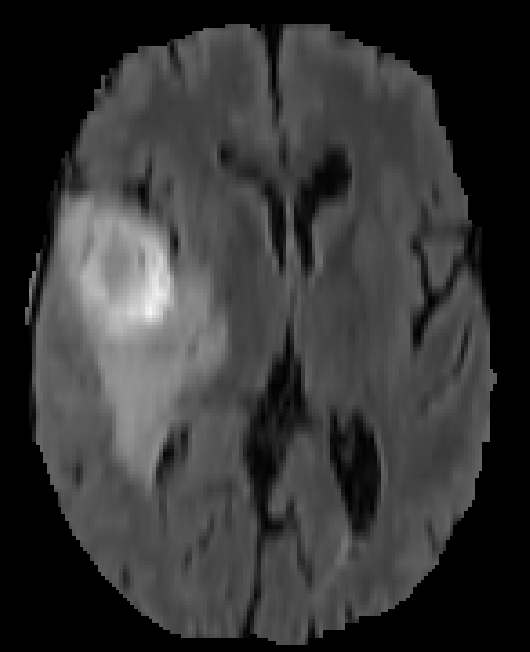
\includegraphics[width=30mm]{Figures/BRATS_HG0001/BRATS_HG0001_FLAIR_slice93.png} &
  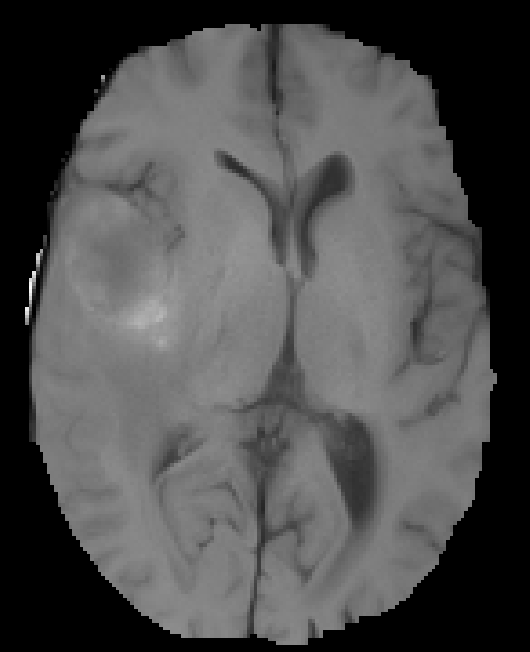
\includegraphics[width=30mm]{Figures/BRATS_HG0001/BRATS_HG0001_T1_slice93.png} &
  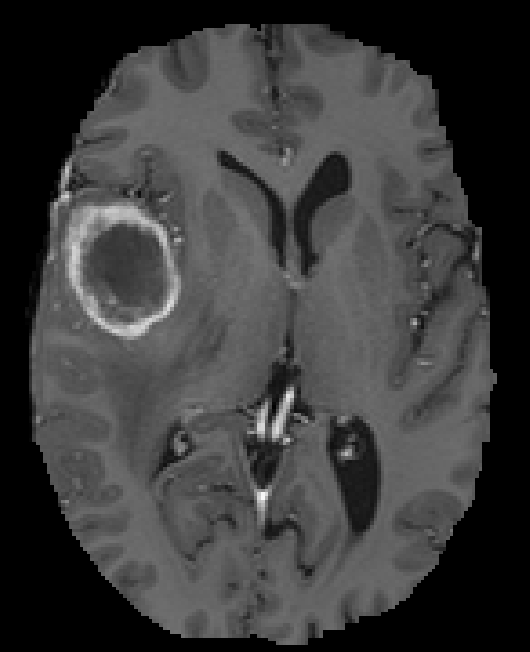
\includegraphics[width=30mm]{Figures/BRATS_HG0001/BRATS_HG0001_T1C_slice93.png} &
  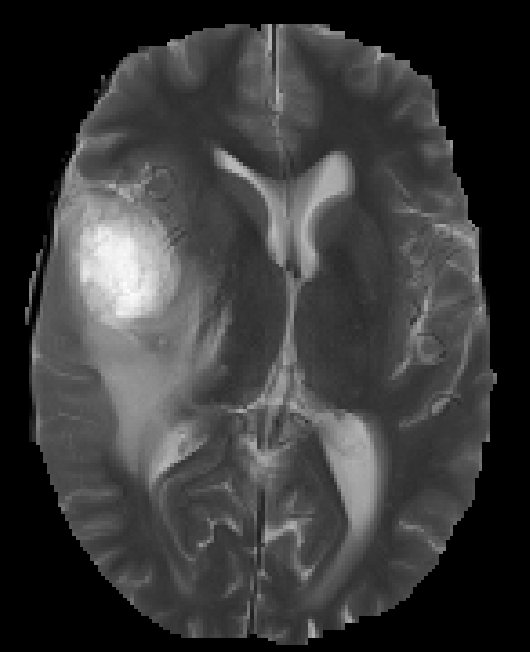
\includegraphics[width=30mm]{Figures/BRATS_HG0001/BRATS_HG0001_T2_slice93.png} \\
  (a) & (b) &
  (c) & (d) \\
  \end{tabular}
  \caption{Induced bilateral asymmetry due to tumor presence causing
  distortion of the plane of symmetry.  Shown are mid-axial slices of
  one of the BRATS 2013 training data 
  (specifically {\tt BRATS\_HG0001}):  (a) FLAIR, (b) T1, (c) T1C, and
  (d) T2.  }
  \label{fig:asymmetry}
\end{figure}

In order to better characterize deviations from normal brain shape 
and appearance, several image features were derived using symmetric 
population-specific multivariate templates.  
For normal neuroanatomy, the use of spatial prior information 
coupled with image normalization capabilities has proven useful 
in producing improved segmentation results of ``expected'' brain tissue
such as cerebrospinal fluid, gray matter, and white matter 
\citep[e.g.,][]{ashburner1997}.  In contrast, accommodating spatial 
priors to model the presence of a possible tumor and its constituent tissue 
components is difficult. However, since the normal brain 
exhibits a bilaterally symmetric organization, we can 
use the presence of asymmetries to potentially differentiate abnormal 
brain tissue.  A similar motivation prompted
the identification of the mid-sagittal plane of symmetry \citep{prima2002}
for feature generation in multiple sclerosis lesion \citep{geremia2011} and 
tumor \citep{geremia2012} identification.  However, this
approach does not take into account the displacement of 
normal tissue due to tumor growth causing the mid-sagittal plane
to deform from its planar structure (cf Figure \ref{fig:asymmetry}).


\begin{figure}[h]
    \centerline{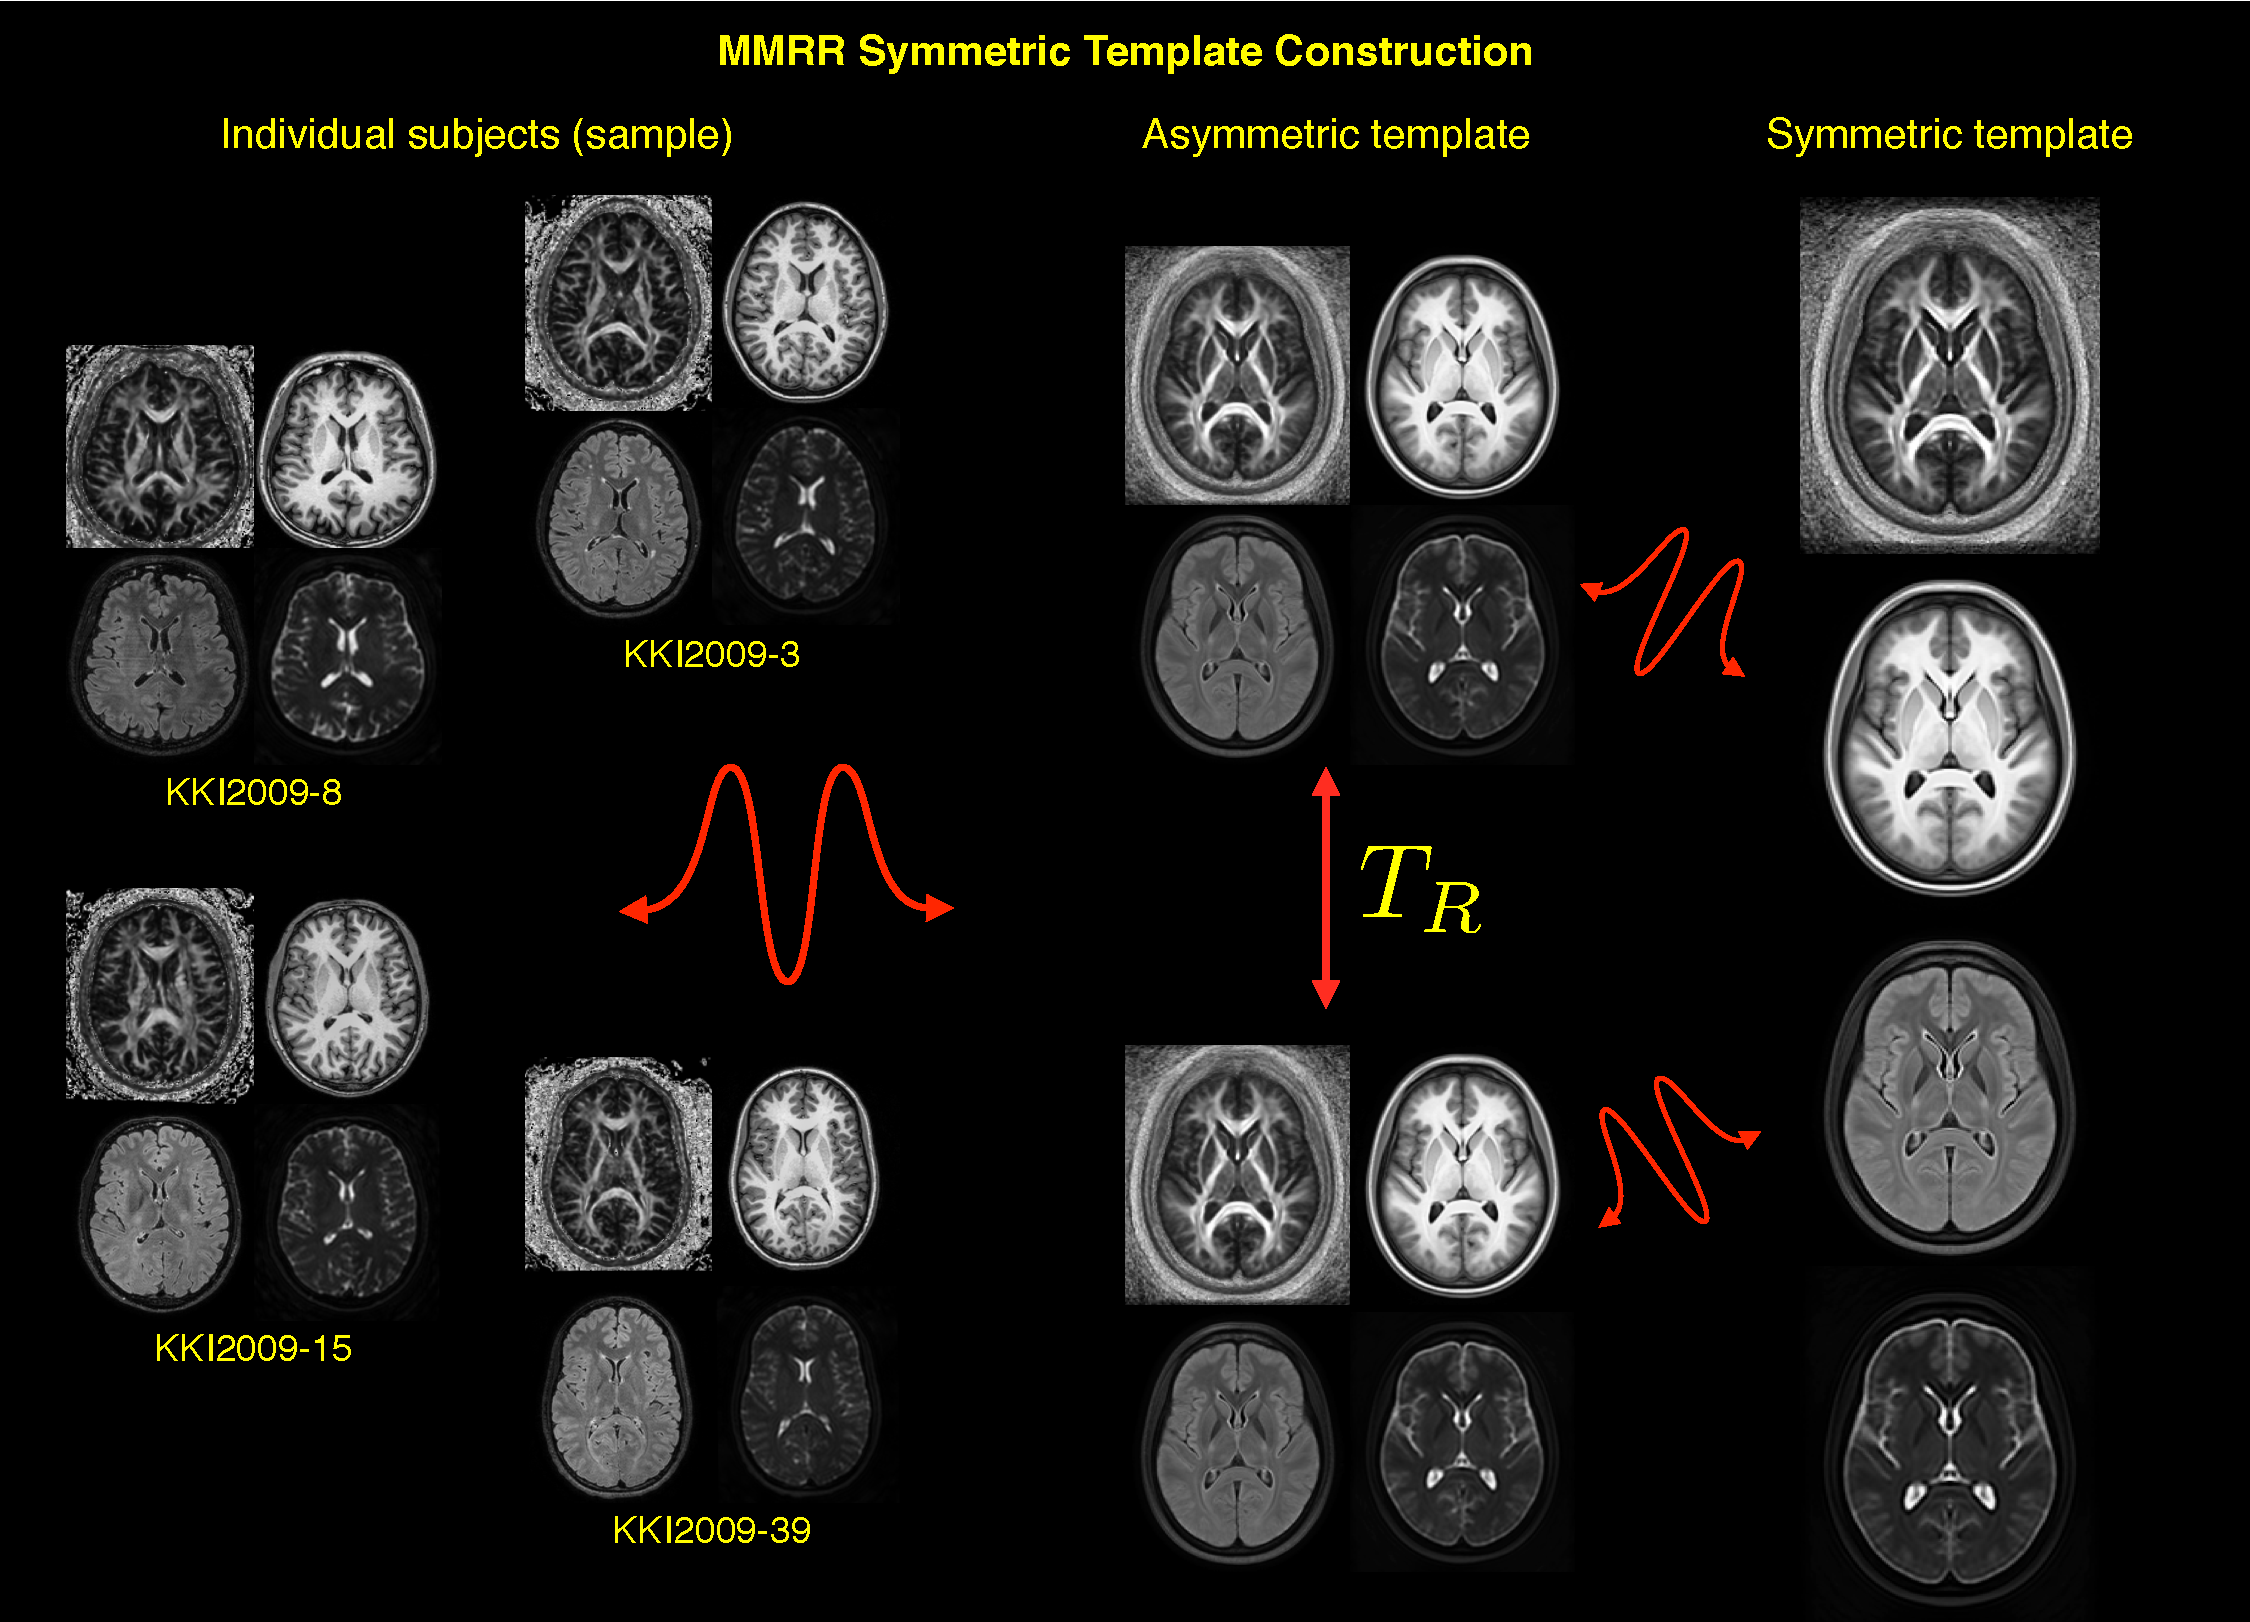
\includegraphics[width=130mm]{Figures/templateKirby.pdf}}
  \caption{Multivariate symmetric template created from the MMRR 
           data \citep{landman2011}.  Of the seven modalities 
           comprising the set of study acquisitions, we illustrate the
           (a) FA, (b) FLAIR, (c) MPRAGE, and (d) T2 template components.
           The optimal transformation and averaging of the individual 
           subject images result in the asymmetric template represented at 
           the top of the middle column.  A horizontal reflection 
           perpendicular to the mid-sagittal
           plane, $T_R$, resulted in the contralateral counterpart represented
           at the bottom of the second column.  The final template seen on
           the right is a result of repeating the template construction using
           the two asymmetric templates as input.
          }
  \label{fig:symmetrictemplates}
\end{figure}


To take into account these potential asymmetries, we 
require a data set with the same modalities as dictated
by the subject image acquisition protocol.  Although it
would be preferable to build population-specific multivariate
templates from normal data using the same acquisition 
parameters \citep{avants2010}, we substituted well-known,
publicly available data since such normal data was not made available
for the BRATS 2013 challenge. 
A recent neuroimaging reproducibility study
by Landman et al. resulted in an open data cohort of 21
normal individuals, each imaged twice, comprising several
modalities including ASL, FLAIR, DTI, fMRI, T1, and T2 
\citep{landman2011}.  These data (known as the
``MMRR'' data set) were selected for deriving
a multivariate template due to its public availability and
inclusion of several modalities (even permitting future 
incorporation of modalities 
not currently included with the BRATS challenge into our 
segmentation framework).  


\begin{figure}[!h]
  \centering
    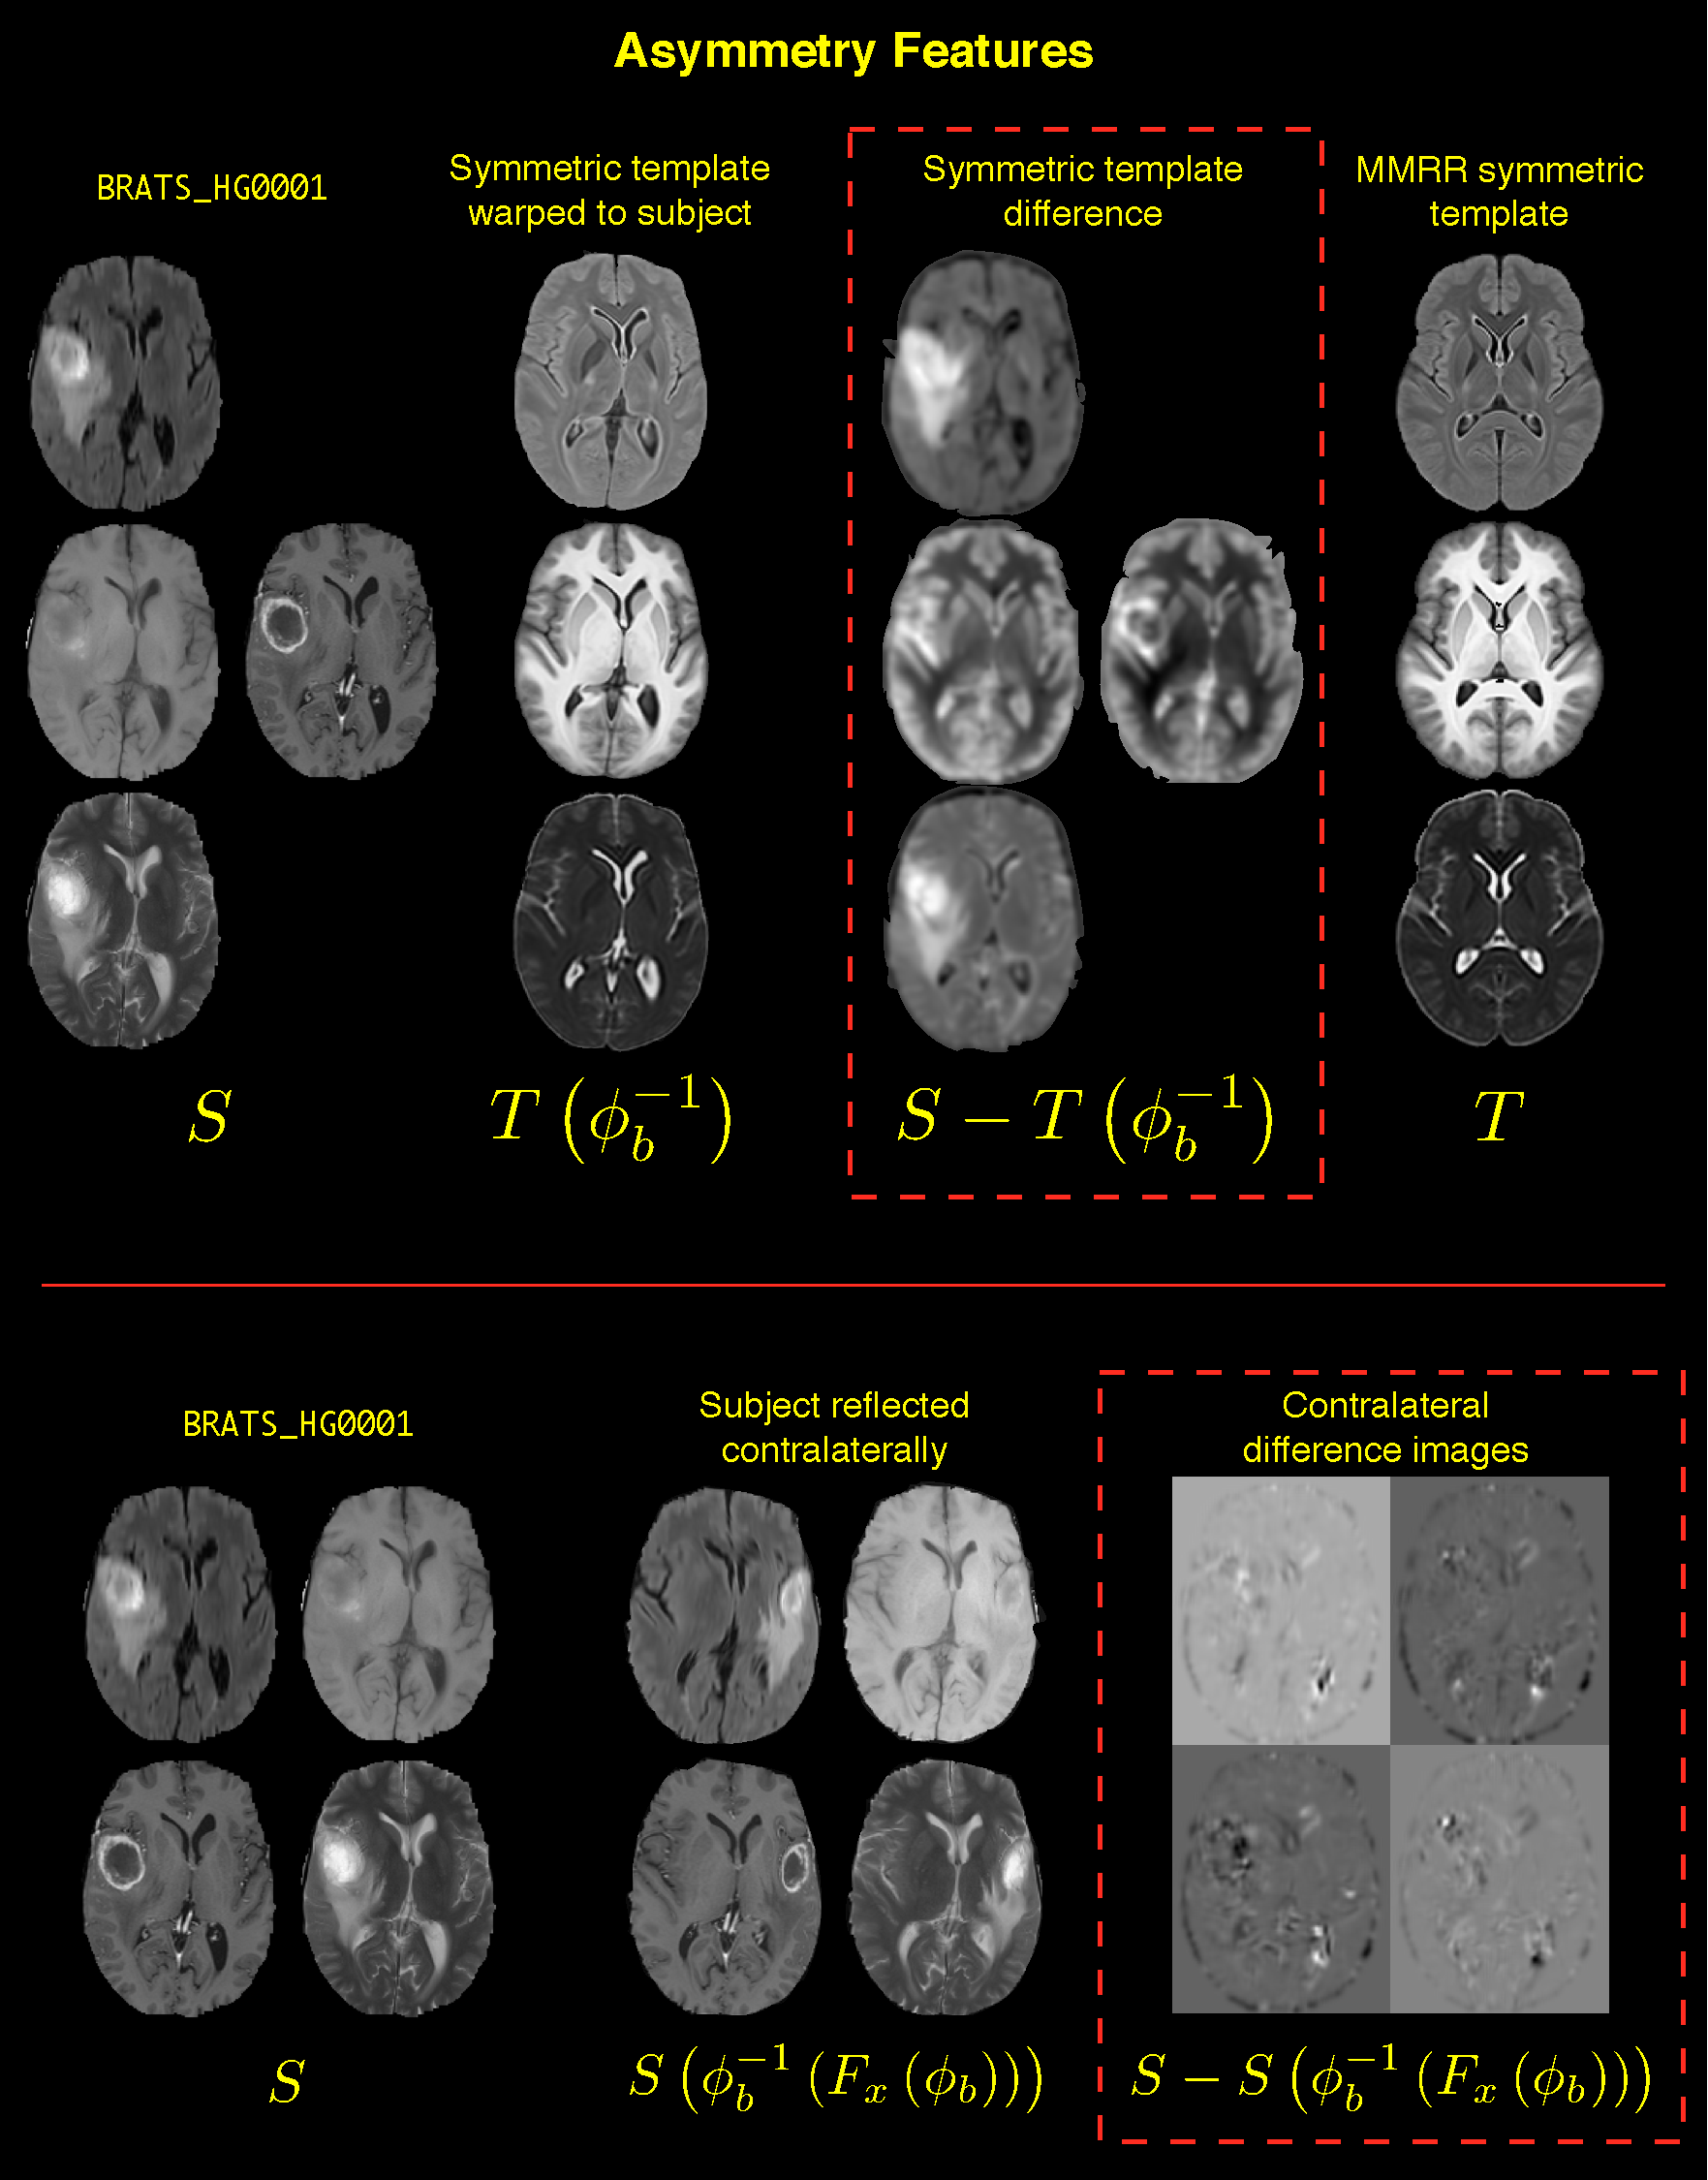
\includegraphics[width=100mm]{Figures/asymmetryFeatureImages.pdf}
  \caption{ Given the mapping between the template, $T$, and subject, $S$, domains ($\phi_b: S  \leftrightarrow \underset{b}{\leftrightsquigarrow} T$), various features can be calculated which demonstrate good discriminative qualities.  Feature images used are outlined in a dashed line.
Top:  Difference images with the symmetric multivariate template are created by warping the template to the subject space and performing a voxelwise subtraction from the original modality image.
Bottom:  Similarly, contralateral difference images are calculated from each modality per subject by generating the non-Euclidean contralateral image via the diffeomorphic transform $\phi_b$.  
          }
  \label{fig:asymmetryFeatures}
\end{figure}

As detailed in \cite{avants2008,avants2010}, 
given $K$ multimodality images, ${\mathbf I} = \{I_1,I_2,\ldots, I_K\}$, 
for $N$ subjects,  multivariate 
template construction iterates between optimizing the set 
of diffeomorphic transforms between the subjects and the 
template, 
$\left\{\left(\phi_1,\phi_1^{-1}\right),\ldots,\left(\phi_N,\phi_N^{-1}\right)\right\}$ 
and constructing the 
optimal multivariate template appearance 
$\mathbf{J}=\{J_1,J_2,\ldots, J_K\}$ to minimize the
following cost function:
\begin{align}
  \sum_{n=1}^N 
        \left[ D \left( \psi(\mathbf{x}),\phi_1^n(\mathbf{x},1)\right)  
        + \sum_{k=1}^K \lambda_k \Pi_k \left(I_k^n\left(\phi_n(\mathbf{x},0.5)\right),J_k\left(\phi^{-1}_n(\mathbf{x},0.5)\right)\right)\right]
\end{align}
$D$ is the diffeomorphic shape distance,
\begin{align}
D\left( \phi( \mathbf{x},0),\phi( \mathbf{x},1)\right) = \int_0^1 \| \nu(\mathbf{x},t)\|_L dt
\end{align}
dependent on the choice of linear operator, $L$, and $\nu$
is the velocity field
\begin{align}
\nu\left( \phi(\mathbf{x},t) \right) = \frac{d\phi(\mathbf{x},t)}{dt},\,\,\, \phi(\mathbf{x},0) = \mathbf{x}.
\end{align}
Each pairwise registration employing the similarity metric $\Pi_k$ can 
be assigned a relative weighting, $\lambda_k$, to weight a particular
modality's influence in the construction process.  Once the multivariate
template has converged (typically in four iterations), we symmetrize
the template by flipping each asymmetric template component contralaterally 
and then running the
multivariate template construction a second time using only the multivariate
template and its symmetric analog.  This is illustrated conceptually in
Figure \ref{fig:symmetrictemplates}.

In terms of implementation, this template building algorithm is 
encapsulated in the script \verb#antsMultivariateTemplateConstruction.sh#,
available in the ANTs repository, which permits serial or parallel processing on
an individual workstation or on a computational cluster.  In
Figure \ref{fig:symmetrictemplates} we show mid-axial slices from
the MMRR multivariate symmetrical template consisting of FA%
\footnote{
Although DWI-based images were not included in the
challenge data, such images have shown discriminative potential 
\citep{price2003,cha2005} warranting investigation in our future
work.  
}, FLAIR,  
T1, and T2 components.  These images have been made publicly available
along with other processed images such as corresponding
tissue priors and structural labels.%
\footnote{
http://figshare.com/articles/Kirby\_multivariate\_template/852989.
All 7 components are stored under the more informal ``Kirby'' data set moniker.
}

After constructing the template offline, each data set is processed
by first registering the non-contrast T1-weighted image to the T1-weighted
component of the symmetric template.  To do this we use a recently developed 
SyN \citep{avants2011a} variant based on B-spline regularization 
which has demonstrated good performance in normal brain registration \citep{tustison2013a}.
Good performance also extends to this pathological data scenario as 
indicated by visual inspection and the fact that the derived features
were amongst the most informative in our winning entry.

We denote the mapping from the subject, $S$, to the template, $T$,
space as $\phi_b: S \leftrightarrow \underset{b}{\leftrightsquigarrow}  T$
which consists of both affine and diffeomorphic components.  Transform
invertibility is essential for the template-based features.  The first 
set of feature images is generated by warping the template components 
to the subject space and calculating the difference image (see the 
top portion of Figure \ref{fig:asymmetryFeatures}).  For example,
the T2 symmetric template voxelwise difference image is calculated from
\begin{align}
  \mathrm{T2}\,\,\mathrm{symmetric}\,\,\mathrm{template}\,\,\mathrm{difference} = S_{\mathrm{T2}} - T_{\mathrm{T2}}\left(\phi_b^{-1}\right).
\end{align}
Note that the T1-weighted contrast and non-contrast images are paired with
the T1-weighted component of the symmetric template.  The second
set of template-based feature images is generated per modality 
as the difference image with the contralateral reflection.  This is achieved by calculating the reflection transform, $T_R$, in the symmetric template space and composing transforms
as follows to create the non-Euclidean contralateral counterpart per modality:
\begin{align}
  S_{contralateral} = S\left( \phi_b^{-1}\left( T_R\left( \phi_b \right)\right)\right).
\end{align}
This process is illustrated in the bottom portion of Figure \ref{fig:asymmetryFeatures}. A final, related feature is the Jacobian
of the transform.  The basis for this final feature is that 
relatively larger Jacobian values might be indicative of tumor
expansion.


\subsubsection{Image Features for Concatenated Random Forests}

\begin{figure}[!h]
  \centering
  \begin{tabular}{c}
    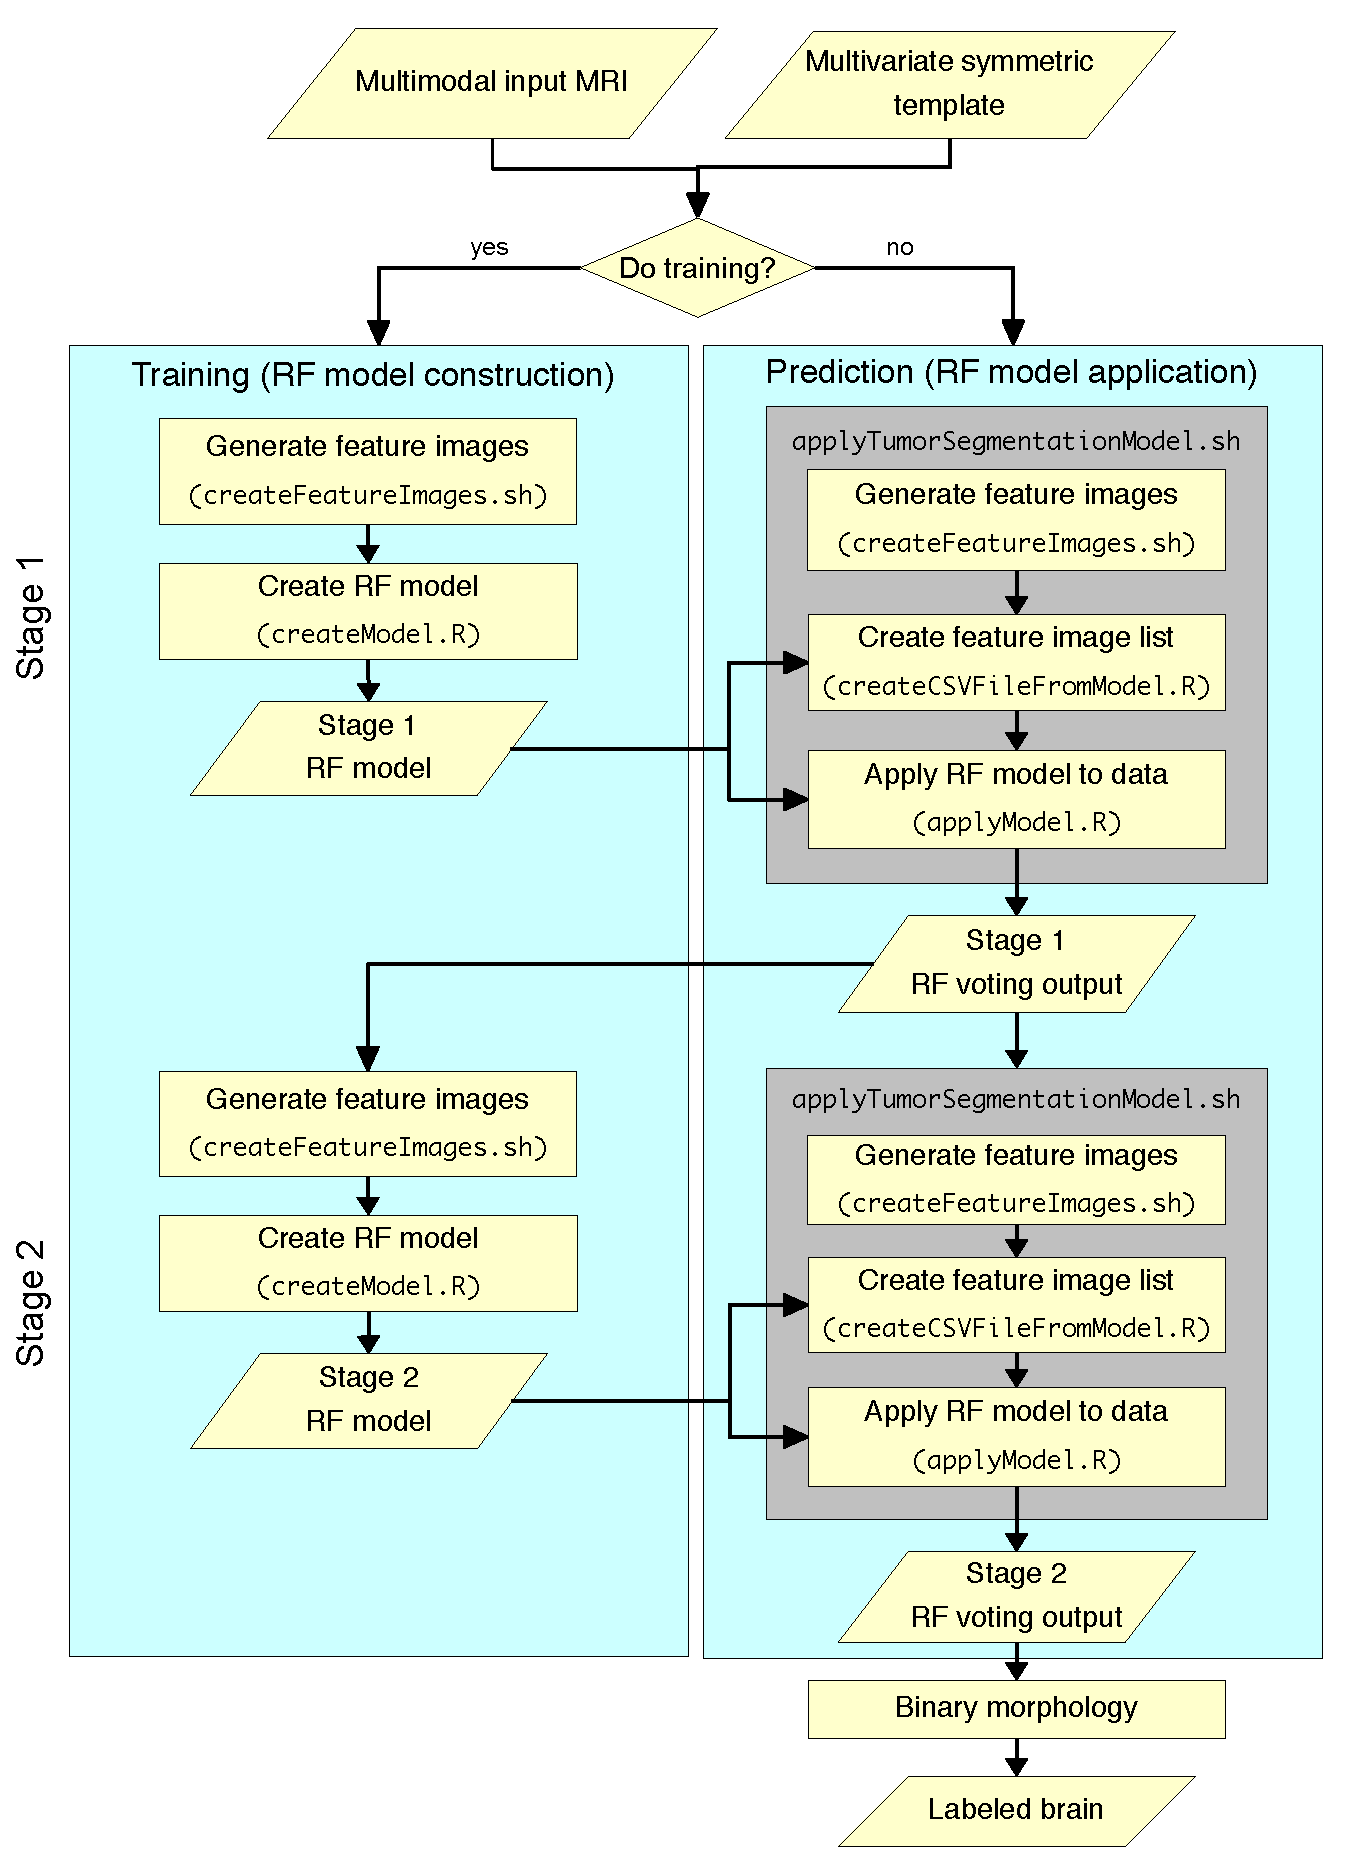
\includegraphics[width=100mm]{Figures/pipeline2.pdf}
  \end{tabular}
  \caption{Diagrammatic workflow for the proposed RF model training and prediction.  The feature
  images are first generated from the input MRI and symmetric multivariate template. If training,
  the set of feature images derived from the training data are used to create the RF model
  for the first stage.  The model is then applied to the training or prediction data to generate 
  a second set of feature images to create the second stage RF model (if training) and/or generate
  the second RF model.  
  For prediction, the final refinement process entails a series of heuristically-derived
  binary morphological resulting in the final labeled brain.  
  }
  \label{fig:pipeline}
\end{figure}


Our segmentation protocol involves training and application
of two RF models in succession 
(see Figure \ref{fig:pipeline}) to which we refer as ``stages.''  The basic idea is that
we generate a set of feature images used as input to the
first RF model (or first stage) which produces a voxelwise 
probabilistic tissue estimate%
\footnote{
More precisely, in the RF framework, each prediction sample (i.e. the feature vector at each voxel),
is propagated through each tree of the ensemble where it is labeled as belonging to a specific
class.  These ``votes'' are converted to voxelwise probabilistic estimates for each class.
}
 for the seven brain/tumor tissue types:
\begin{itemize}
\item cerebrospinal fluid,
\item grey matter,
\item white matter,
\item edema, 
\item non-enhancing tumor (including low-grade tumor center), 
\item enhancing tumor (excluding necrotic center), and 
\item abnormal necrotic center or necrocyst in high-grade gliomas.
\end{itemize}
We then use these output tissue map estimates as spatial 
priors for generating a second set of image features.  These
are used as input for a second RF model application (or
second stage),
the output of which constitute the final tumor segmentation estimate.
Note that some feature images are included in both stages such as
the asymmetry features described in the previous section.

For both stages, in contrast to previous generative
modeling approaches for multimodal tumor segmentation 
\citep[e.g.,][]{prastawa2003}, we do not use multivariate 
Gaussians to specify tissue probabilities but rather incorporate each
univariate probability map into the feature vector of the training
data.  As pointed out in \cite{menze2010}, multivariate modeling
might obscure the distinct biological information provided by each 
modality.  Instead, we let the RF construction 
process determine the optimal combination of such multivariate
information.  Additionally, maximum posterior labeling from both stages
is used to determine the connected components for each label.  
Geometric features (assigned voxel-wise) include the physical volumes 
of each connected component, the volume to surface area ratio, 
the elongation, and eccentricity. 

\paragraph{Stage 1 (GMM)}
Gaussian mixture modeling (GMM) is used to assign voxelwise
tissue probabilities which comprise an additional set of image features 
where 
prior cluster centers for specific tissue types for each
modality are learned from training data \citep{reynolds2009}.  
Intensity normalization
across the training cohort was originally performed using 
\cite{nyul2000}.  However, despite good performance on normal
data, application of this intensity normalization algorithm 
(after a thorough parameter search) on BRATS data led to slightly 
worse performance than simply winsorizing the intensity values to the quantile
range $[0.01, 0.99]$ and then rescaling the resulting intensities to 
$[0,1]$ so we opted for the latter, more simplistic intensity
normalization protocol.  The cluster centers are defined as the mean
normalized intensity value for each tissue type of each modality 
image over all the training data.  It should be noted that 
initializing with these values is optional and that results
seem to be robust to initialization values.

A GMM formulates the 
probability distribution at each voxel, $\mathbf{x}$, as the
sum of $M$ Gaussian components, $\mathcal{N}(\mathbf{x}|\mu,\sigma)$, i.e.
\begin{align}
p\left(\mathbf{x}|\mu_m,\sigma_m,\lambda_m\right) = \sum_{i=1}^M \lambda_m \mathcal{N}(\mathbf{x}|\mu_m,\sigma_m)
\end{align}
where $\sum_{m=1}^M \lambda_m = 1$.  The parameters of the GMM 
are determined with maximum likelihood estimation using the 
Atropos segmentation tool \citep{avants2011} available in ANTs.  
We include the resulting seven posterior probability tissue images 
along with five additional geometric features based on the connected 
components of the segmentation image (distance image to tumor core,
physical volume image, volume to surface area ratio, eccentricity,
and elongation).
During the training phase (or RF model construction),
these feature images, $\left\{F_i: i \in GMM\right\}$, generated during Stage 1 are used to create
the Stage 1 RF model using the following relationship
\begin{align}
\label{eq:gmm}
\mathrm{Tissue}\,\,\mathrm{classes} \sim \sum_{i \in GMM} F_i + \sum_{i \in Asym} F_i + \sum_{i \in Misc} F_i
\end{align}
given in the standard R notation of \cite{wilkinson1973}.  The
set of $\left\{F_i: i \in Asym\right\}$ are the feature images 
generated from the symmetric multivariate template 
described in the previous section and $\left\{F_i: i \in Misc\right\}$
are miscellaneous  feature images described in Section \ref{sec:misc}.

\paragraph{Stage 2 (MAP-MRF)}

Application of the Stage 1 RF model results in a set of
probabilistic estimates for each of the seven tissue types.  
At the beginning of the second stage, these spatial probability maps are 
used as spatial priors in a 
MAP-MRF segmentation also performed using the Atropos 
segmentation tool \citep{avants2011} available in ANTs although we couple
it with N4 bias correction \citep{tustison2010} as contained in the script
{\tt antsAtroposN4.sh}.  The probabilistic segmentation output and corresponding
connected-component feature images for each modality replace the analogous 
GMM-based feature images used 
during the first stage of training/prediction along with the other feature
images generated during the feature stage (such as the template-based data).
The second stage RF model is then produced similarly as the previous stage: 
\begin{align}
\label{eq:mapmrf}
\mathrm{Tissue}\,\,\mathrm{classes} \sim \sum_{i \in MAP-MRF} F_i + \sum_{i \in Asym} F_i + \sum_{i \in Misc} F_i.
\end{align}
We discovered that this composite application of random
forest models improves the resulting labeled output.

\subsubsection{Miscellaneous Multimodal Feature Image Generation}
\label{sec:misc}

In addition to the feature images outlined in the previous sections, 
several other feature images were generated largely based on what 
had been used in previous work.  For each modality, several images
were generated based on calculation of voxelwise neighborhood 
first-order statistics including mean, variance, skewness, and entropy
using neighborhood block radii
of 1 and 3 voxels.  We also calculated two Euclidean distance
transforms \citep{maurer2003} to be used for each subject.  One was
calculated from the subject's own cerebral mask and the other was the 
distance transform of the symmetric template cerebral mask warped
to the subject.  Finally, we also generated the  (T1 - T1C) difference 
image \citep{prastawa2003}.
The script {\tt createFeatureImages.sh} performs all preprocessing
and generates all feature images.  In Figure \ref{fig:featureImages} we provide sample mid-axial 
image slices from features generated from the {\tt BRATS\_HG0301} data set.

\begin{figure*}[h]
%  \centering
%  \makebox[0.9\textwidth][c]{
  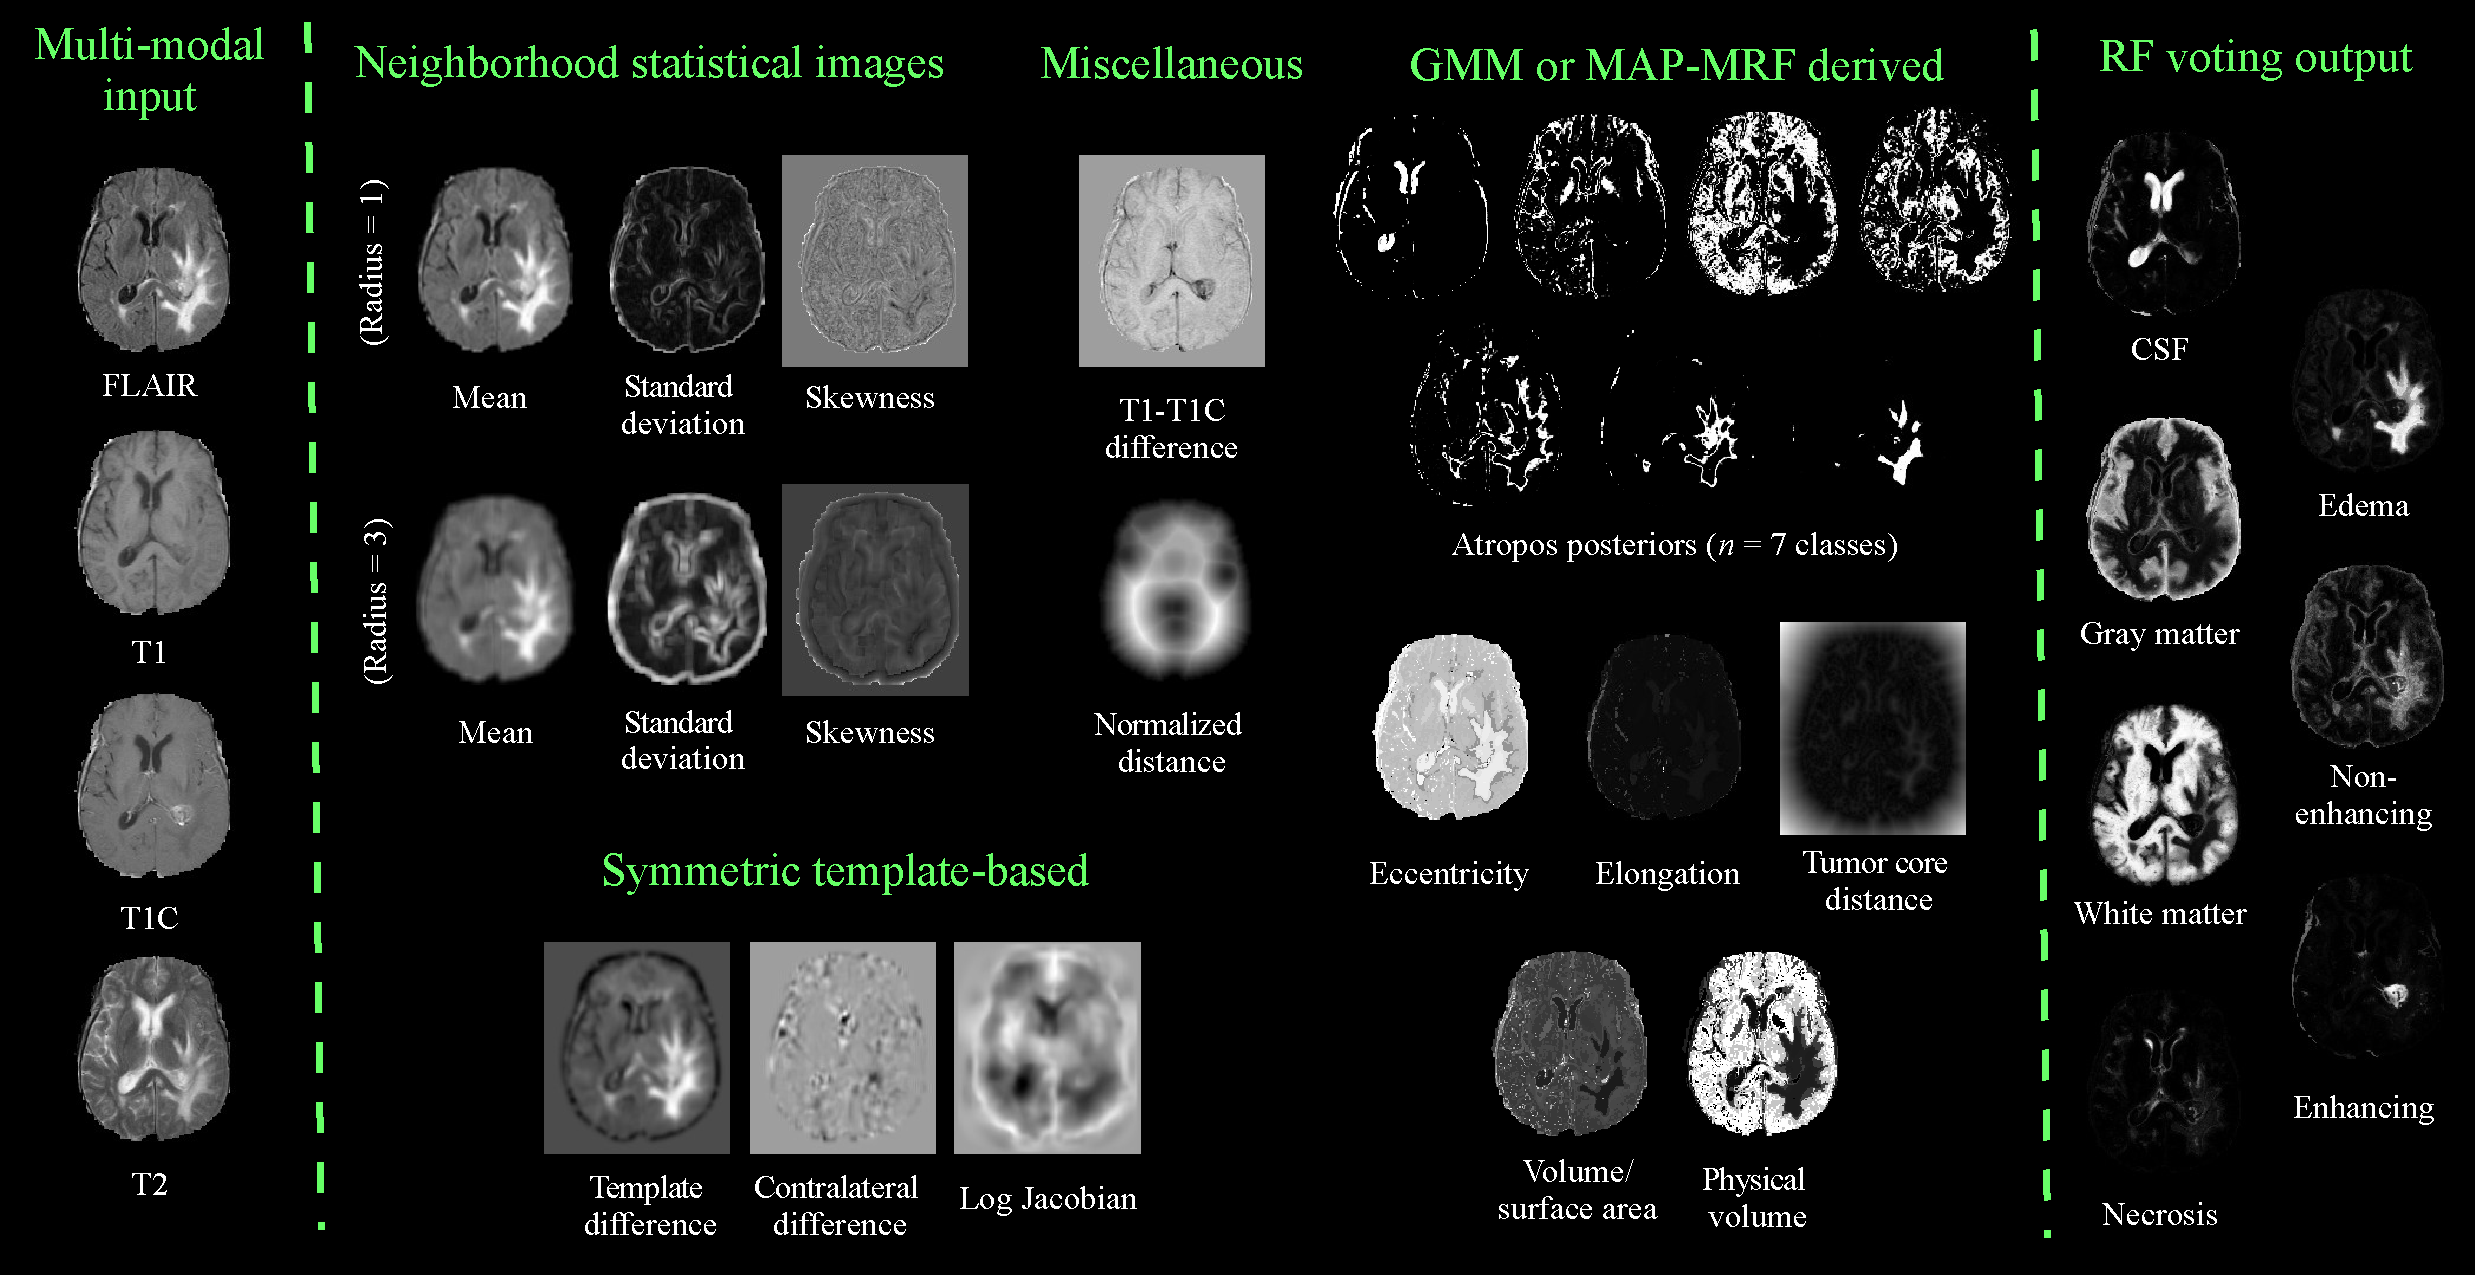
\includegraphics[width=150mm]{Figures/featureImages.pdf}
%  }
  \caption{Representative feature images derived from the 
           BRATS\_HG0301  ``challenge'' data set.
           Neighborhood statistical images for each modality were 
           generated by calculating a given statistic within
           a specified neighborhood radius.  Also calculated for each modality were feature
           images based on either the GMM or the MAP-MRF segmentation.  For the former, we
           show the probability maps for each of the seven labels which are used as feature
           images.  From the resulting hard segmentation, we calculate various geometric 
           measures per connected component of each of the seven labels.  Similarly, the 
           registration to the symmetric template produces the modality-specific 
           difference images with the
           corresponding symmetric template itself and with respect to the 
           contralateral side.   
           This mapping is also used to produce the log Jacobian image.  Finally, the 
           (T1 - TC) image is calculated and, from the
           cerebral mask, we calculate the normalized distance image.  
           }
  \label{fig:featureImages}         
\end{figure*}


\subsection{\textit{ANTsR}:  An ANTs/R Interface}

\subsubsection{Overview}

The complexity of neuroimaging research necessitates 
commensurable numerical analysis capabilities.  Similarly, concomitant
with the era of ``big data'' (specifically with respect to neuroimaging
\citep{vanhorn2013}) are new visualization needs and challenges
\citep{childs2013,kehrer2013}.
In response, various software packages have been developed to
integrate tools specific to neuroimaging research with more general
numerical and visualization software packages.
The well-known neuroimaging package SPM%
\footnote{
http://www.fil.ion.ucl.ac.uk/spm/
}
is a significant extension of the commercial computing and visualization environment
Matlab.  Open source neuroimaging packages, such as NIPY (neuroimaging in Python),%
\footnote{
http://nipy.org
} 
rely on other open source packages for numerical/statistical analysis.  NIPY,
for example, uses the more generic packages NumPy and SciPy for numerical analysis and 
optimization.%
\footnote{
http://www.numpy.org
}  

ANTs (Advanced Normalization Tools) was built, originally, to provide 
high performance image registration for medical image analysis
\citep{avants2008a} and based upon the mature Insight Toolkit (ITK)
sponsored by the National Institutes of Health.  Since then, ANTs has grown to include 
several robust medical image analysis solutions including bias 
correction \citep{tustison2010}, $n$-tissue multivariate segmentation 
\citep{avants2011}, template construction \citep{avants2010}, and cortical 
thickness estimation \citep{das2009} (many of which have been
introduced into ITK partially in an attempted leveraging of Linus's Law---``Given enough eyeballs, all bugs are shallow'').  
However, in the evolution of the toolkit, it became clear 
that robust statistical machinery was lacking for making inferences regarding
the data produced during the course of ANTs processing.  \textit{ANTsR} was developed
specifically to provide an interface between ANTs, a 
powerful neuroimaging toolkit for producing reliable imaging data 
transformations, and the R project%
\footnote{
http://www.r-project.org
}
for statistical computing and visualization thus providing a complete
set of tools for multivariate neuroimage analysis.  
 \textit{ANTsR} intends to provide a modern framework for medical analytics, 
 with a focus on imaging-assisted prediction and statistical power.


Careful consideration of available statistical software 
led to the adoption of R to complement ANTs quantification resulting in the
\textit{ANTsR} package.
%The R project for statistical computing,%
%\footnote{
%www.r-project.org
%}
% or more compactly
%`R', is an environment for statistical computation
%and data visualization.  
R's open source code base, reliable software testing and distribution strategies,
and add-on packages coupled with its rapidly growing 
community of developers and users has caused wide-scale
adoption within both academia and industry.

\subsubsection{Installation}

The \textit{ANTsR} package is publicly available on the github project hosting service.%
\footnote{
\href{https://github.com/stnava/\textit{ANTsR}}{https://github.com/stnava/\textit{ANTsR}}
}
Prior to installation of \textit{ANTsR}, several external R packages
need to be installed including: \verb#Rcpp#, \verb#signal#, \verb#timeSeries#, 
\verb#mFilter#, \verb#doParallel#, \verb#robust#, \verb#magic#, \verb#knitr#, \verb#pixmap#, 
\verb#rgl#, and \verb#misc3d#.%  
\footnote{
See \href{http://stnava.github.io/software/2014/01/08/antsr/}{http://stnava.github.io/software/2014/01/08/antsr/} for current status.}
Additionally, in order
to perform the supervised brain segmentation as described 
in later sections, one needs to also install the packages
\verb#randomForest#, \verb#snowfall#, \verb#rlecuyer#,
and \verb#ggplot2#.%
\footnote{
Packages are easily installed using the {\tt install.packages()} R mechanism.
} 

In addition to R and the add-on packages previously mentioned, CMake is also 
required.  CMake%
\footnote{
http://www.cmake.org/
}
is an open source tool for the management and building of 
large-scale software projects.  It is used
to coordinate the downloading of external packages,
such as the Insight Toolkit (ITK)%
\footnote{
http://www.itk.org/
}
and ANTs.  Further instructions for download and
installation can be found on the \textit{ANTsR} github website.  Feel
free to contact the authors if installation trouble occurs.  We note
that \textit{ANTsR} is currently only tested on UNIX-alikes such OSX and Ubuntu
operating systems.%  
\footnote{Windows installation should be possible
but, to our knowledge, has not been attempted.}

\subsubsection{Usage}
\textit{ANTsR} is intended to not only allow easy interchange between
medical imaging formats and R but also to facilitate
reproducible scientific studies and the type compilable analysis
articles that are fundamental to journals such as
\textit{Biostatistics}.  Both \verb#knitr# and \verb#sweave#
facilitate integration of R-code with the LaTeX document
preparation system.  

An additional motivation for our development of \textit{ANTsR} (and
hopefully its acceptance by the community) 
stems from the ability to couple ANTs core 
functionality, including IO tools such as \verb#antsImageRead#, 
with the large number of R statistical and
visualization packages.  Due to this combination, several
functions have been easily created for such neuroimaging-specific 
tasks as fMRI/ASL data manipulation and analysis,
voxel and ROI-based  analyses,
%(e.g. \verb#filterMRIforNetworkAnalysis#, \verb#aslPerfusion#)
and connectivity visualization. % (e.g. \verb#plotBasicNetwork#).
The user help menu and documentation for the library  and its
constituent functions are invoked in the similar manner as other
R libraries.

As mentioned earlier, we have made this entire framework
available as open source.  In addition to the \textit{ANTsR} repository
already on github which houses both ANTs and \textit{ANTsR} functionality, 
we created a special github repository specifically for this work
containing figures, references, and text.%
\footnote{
\href{https://github.com/ntustison/ANTsAndArboles}{https://github.com/ntustison/ANTsAndArboles}
}
Also, we posted all
scripts (R, shell, and perl) used to coordinate the \textit{ANTsR} processing 
including:
\begin{itemize}
  \item {\tt applyModel.R}:  applies a RF model to a new 
  feature data set from a testing subject resulting in a set of probability
  images (one for each label).
  \item {\tt applyTumorSegmentationModel.sh}:  generates the new feature image set 
  from the testing MRI (by calling {\tt createFeatureImages.sh}).
  organizes the file names in a csv file (via {\tt createCSVFileFromModel.R}),
  and applies the RF model using {\tt applyModel.R}. 
  \item {\tt applyTumorSegmentationModelForCohort.pl}:  Coordinates tumor 
  segmentation on the computational cluster for a given cohort.
  \item {\tt createCSVFileFromModel.R}:  organizes the set of feature image
  file names in a csv file for input into {\tt applyModel.R}.
  \item {\tt createFeatureImages.sh};  creates the set of feature images given
  a set of co-registered input MRI from a single subject. 
  \item {\tt createModel.R}:  creates a RF model given the input csv 
  file of the feature image file names for all training data and set of truth
  label maps.
  \item {\tt plotVariableImportance.R}:  produces a plot of the importance 
   of each feature variable used 
  in constructing the model.
\end{itemize}
We also include a fully functional 2-D example which performs
both testing and training on sample challenge data.%
\footnote{
https://github.com/ntustison/ANTsAndArboles/tree/master/SimpleExample
}
After pulling the repository, one can run the scripts {\tt exampleTrain.sh}
and {\tt examplePredict.sh} to get the sample results.  Output includes
several overlap measures describing the performance.

\subsection{Brain Tumor Data}

Brain tumor image data used in this work were obtained from the NCI-MICCAI 2013 
Challenge on Multimodal Brain Tumor Segmentation%
\footnote{
http://martinos.org/qtim/miccai2013/index.html
}
organized by K. Farahani, M. Reyes, B. Menze, E. Gerstner, J. Kirby and J. Kalpathy-Cramer. 
The challenge database contains fully anonymized images from the following institutions: 
ETH Zurich, University of Bern, University of Debrecen, and University of Utah and 
publicly available images from the Cancer Imaging Archive (TCIA).  Both training 
and testing data were made freely available through the Creative Commons Attribution-NonCommercial 3.0 license.

Training data consisted of multimodal brain MRI (T1, T2, FLAIR, and 
post-Gadolinium T1) from 30 glioma patients (both low, $n=10$, and high-grade, $n=20$,
and with and without resection).  For each subject, the T1, T2, and 
FLAIR MRI were linearly registered to the post-contrast T1.  Subsequently,
the brains were skull-stripped and resampled to 1 mm isotropic resolution.
Testing data was processed similarly and released during the course of the
challenge in two sets denoted as ``Leaderboard'' and ``Challenge'' data.  
The former consisted of 21 and 4 high and low-grade tumor patients, respectively,
whereas the latter comprised 10 high-grade only patients.

Manual labeling was performed in the axial plane following a detailed
protocol.%
\footnote{
http://martinos.org/qtim/miccai2013/data.html
}
The labeling of pathology was categorized into four regions:
edema, non-enhancing tumor (including low-grade tumor center), 
enhancing tumor (excluding necrotic center), and abnormal
necrotic center or necrocyst in high-grade gliomas.
Normal brain tissue was not labeled. 

\subsubsection{Training: RF Creation for the BRATS 2013 Challenge}

For use with the Challenge and Leaderboard data, cohort-specific models (both 
low-grade and 
high-grade glioma) for both GMM and MAP-MRF stages were created using only the 
supplied training data.  Prior to training, we segmented normal brain tissue \citep{avants2011}
for each data set by segmenting only the T1 image.  This was only to yield
a rough estimate of normal brain tissue to augment the already provided 
pathology labels.  This resulted in seven labels for tissues described
earlier i.e., csf, gray matter, white matter,
necrosis, edema, enhancing, and non-enhancing tumor characterizing each brain.

Initial testing of our proposed framework was performed 
on the training data using a leave-one-out strategy.  Once the
feature images are created for each subject, the resulting images of the entire
training cohort are organized in a csv file for input into the R script
{\tt createModel.R}.  Other possible input parameters include the requested 
number of trees, number of samples per label, and number of threads for parallel
processing.  The output is an {\tt RData} file describing the RF
model which can be used for future predictions.
 
Additionally, the {\tt randomForest} package provides  measurements 
for determining the importance of chosen features when constructing the model.  
This aids in potential feature pruning or intuiting model behavior.  As mentioned
earlier, we provide the R script {\tt plotVariableImportance.R} to render
one such quantity denoted as {\tt MeanDecreaseAccuracy}.  During model construction
(specifically the out-of-bag error calculation stage), the decrease in prediction accuracy
with the omission of a single feature or variable is tracked and averaged.  Thus,
those features which have the greatest decrease in mean accuracy are considered
to be the most discriminative.%
\footnote{
There is an issue with consistently ranking correlated predictors as described at {\tt http://www.r-bloggers.com/random-forest-variable-importance/} since the permutation testing performed for predictive accuracy assessment assumes predictor independence.  Correctives have been proposed but we ignore these issues for this particular application.
}
In this work, we do not use these measurements for feature pruning.  However,
we plot them in the Results section (see Figures \ref{fig:hgimportance} and
\ref{fig:lgimportance}) as they demonstrate the relative importance of our
selected features including that of the proposed asymmetry images.

\subsubsection{Prediction:  Applying the RFs for the BRATS 2013 Challenge}

Once the models are created, classification of tumors in new subjects is performed
as illustrated in Figure \ref{fig:pipeline}.  From the feature images and input 
GMM model, a tentative set of RF voting output confidence images are produced.
As described, this is used as input to the second prediction round.  The 
final probability output images are used to produce the maximum probability labeling.  

A final round of binary morphological operations were heuristically designed
to improve the final segmentation results such as removal of small connected 
components and morphological closure of certain regions.
All steps are included in the script 
{\tt applyTumorSegmentationModelForCohort.pl} designed for parallel subject 
processing on the computational cluster at the University of Virginia.%
\footnote{
http://www.uvacse.edu
}




%%%%%%%%%%%%%%%%%%%%%%%%%%%%%%%%%%%%%%%%%%%%%%%%%%%%%%%%%%%%%%%%%%%%%
%
% Results
%
%%%%%%%%%%%%%%%%%%%%%%%%%%%%%%%%%%%%%%%%%%%%%%%%%%%%%%%%%%%%%%%%%%%%%

\section{Results}


\begin{figure}[!htb]
  \centering
  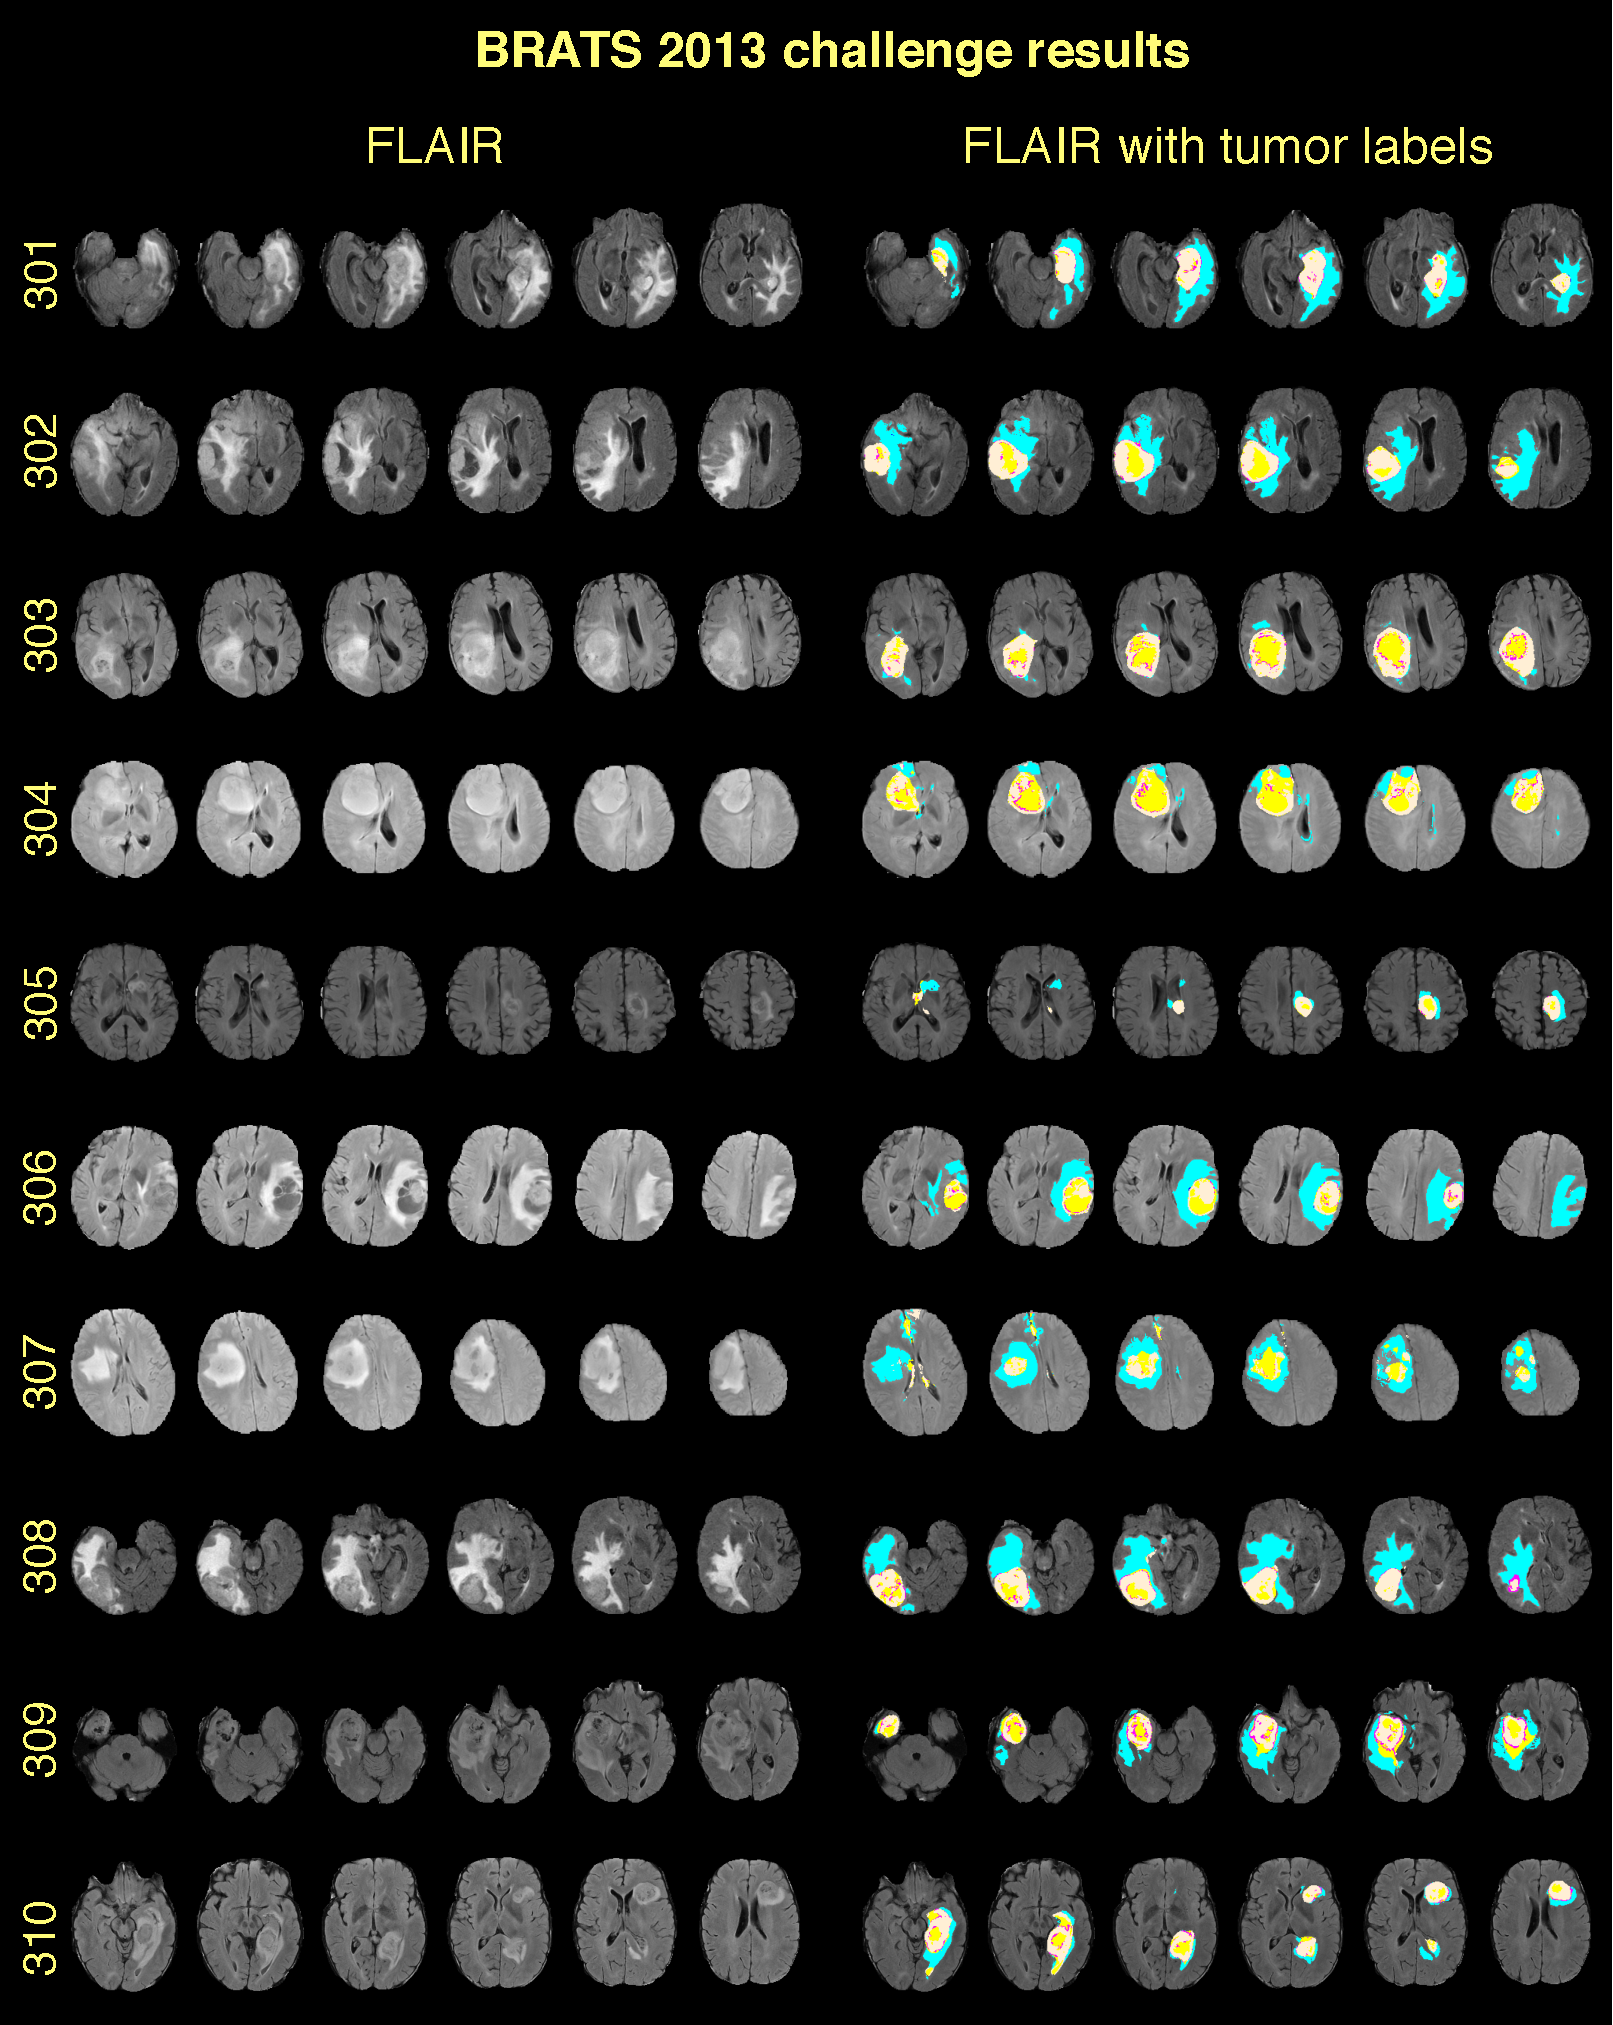
\includegraphics[width=120mm]{Figures/challengeResults.pdf}
  \caption{Visual results (every tenth slice sampled from the axial center of the
  tumor region) from the BRATS 2013 challenge using the proposed
  framework (off-white = non-enhancing tumor, cyan = edema, violet = enhancing 
  tumor, yellow = necrosis).  Tumor components were combined into
  three regions for performance assessment ((1) complete tumor: all four tissue
  classes; (2) tumor core:  necrosis, non-enhancing tumor, and enhancing tumor;
  and (3) enhancing tumor).  See Table \ref{table:results} for quantitative measures
  and challenge rankings.
  }
  \label{fig:challengeresults}
\end{figure}




%\begin{table*}
%\caption{Results from the MICCAI 2013 BRATS Challenge}
%\label{table:results}
%\begin{center}
%\begin{tabular*}{0.99\textwidth}{@{\extracolsep{\fill} } c c c c c c c c c c c}
%\toprule
%{\bf Data set} & {\bf Rank} & \multicolumn{3}{c}{\bf Dice} & \multicolumn{3}{c}{ \bf Positive Predictive Value} & \multicolumn{3}{c}{ \bf Sensitivity} \\
%{} & {} & complete & core & enhanced & complete & core & enhanced & complete & core & enhanced \\
%\midrule
%Challenge & 1 & 0.87 (1) & 0.78 (1) & 0.74 (1) & 0.85 (2) & 0.74 (5) & 0.69 (4) & 0.89 (2) & 0.88 (1) & 0.83 (1) \\
%Leaderboard & 1 & 0.79 (2) & 0.65 (1) & 0.53 (3) & 0.83 (1) & 0.70 (2) & 0.51 (3) & 0.81 (4) & 0.73 (2) & 0.66 (2) \\
%Evaluation & 2 & 0.88 (2) & 0.76 (2) & 0.55 (3) & 0.88 (3) & 0.80 (5) & 0.65 (3) & 0.89 (3) & 0.79 (3) & 0.53 (3) \\
%\bottomrule
%\end{tabular*}
%\end{center}
%\end{table*}


\begin{table*}
\caption{Assessment measures from the MICCAI 2013 BRATS Challenge including
 Dice overlap, positive prediction value (PPV), and sensitivity.}
\label{table:results}
\begin{center}
\begin{tabular*}{0.99\textwidth}{@{\extracolsep{\fill} } l c c c c}
\toprule
\multicolumn{1}{c}{ \bf Data Set} & {\bf Rank}$^\dagger$ & {\bf Dice} & {\bf PPV} & {\bf Sensitivity} \\
\midrule
Challenge (complete) & 1 & 0.87 (1) & 0.85 (2) & 0.89 (2) \\
Challenge (core) & {} & 0.78 (1) & 0.74 (5) & 0.88 (1) \\
Challenge (enhanced) & {} & 0.74 (1) & 0.69 (4) & 0.83 (1) \\
\midrule
Leaderboard (complete) &  1 & 0.79 (2) & 0.83 (1) & 0.81 (4) \\
Leaderboard (core)     & {} & 0.65 (1) & 0.70 (2) & 0.73 (2) \\
Leaderboard (enhanced) & {} & 0.53 (3) & 0.51 (3) & 0.66 (2) \\
\midrule
Evaluation (complete) &  2 & 0.88 (2) & 0.88 (3) & 0.89 (3) \\
Evaluation (core)     & {} & 0.76 (2) & 0.80 (5) & 0.79 (3) \\
Evaluation (enhanced) & {} & 0.55 (3) & 0.65 (3) & 0.53 (3) \\
\bottomrule
\multicolumn{5}{l}{\scriptsize$^\dagger$Indicates performance
for all measures over all regions.  Component rankings are 
given in parentheses.
}
\end{tabular*}
\end{center}
\end{table*}


A total of four RF models were created from the 30 training data 
sets. Two models for Stage 1 and Stage 2 processing were generated from the 
20 high-grade glioma evaluation data described earlier.  Similarly, two
additional models were created from the 10 low-grade glioma data sets.  Following
model construction, weighted importance feature plots described earlier were 
rendered to provide feedback as to the individual potential predictive accuracy
of each feature.  The high-grade plots are given in Figure \ref{fig:hgimportance}
whereas the low-grade plots are given in Figure \ref{fig:lgimportance}.

\begin{figure*}
  \makebox[\textwidth][c]{
  \begin{tabular}{cc}
  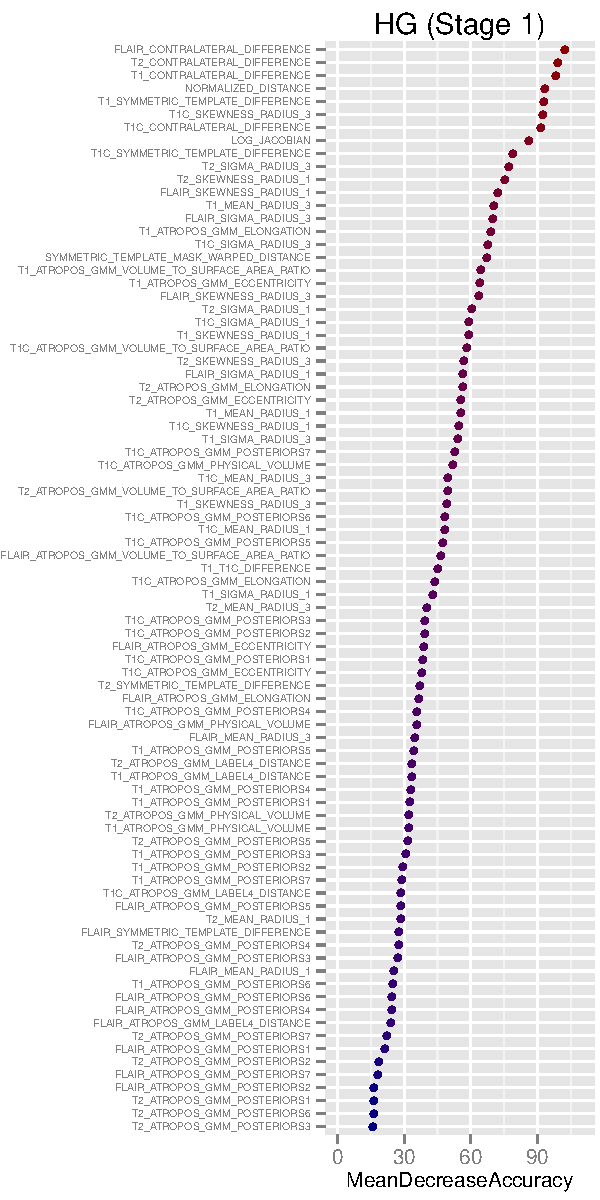
\includegraphics[width=90mm]{Figures/BRATS_HG_GMM.pdf} &
  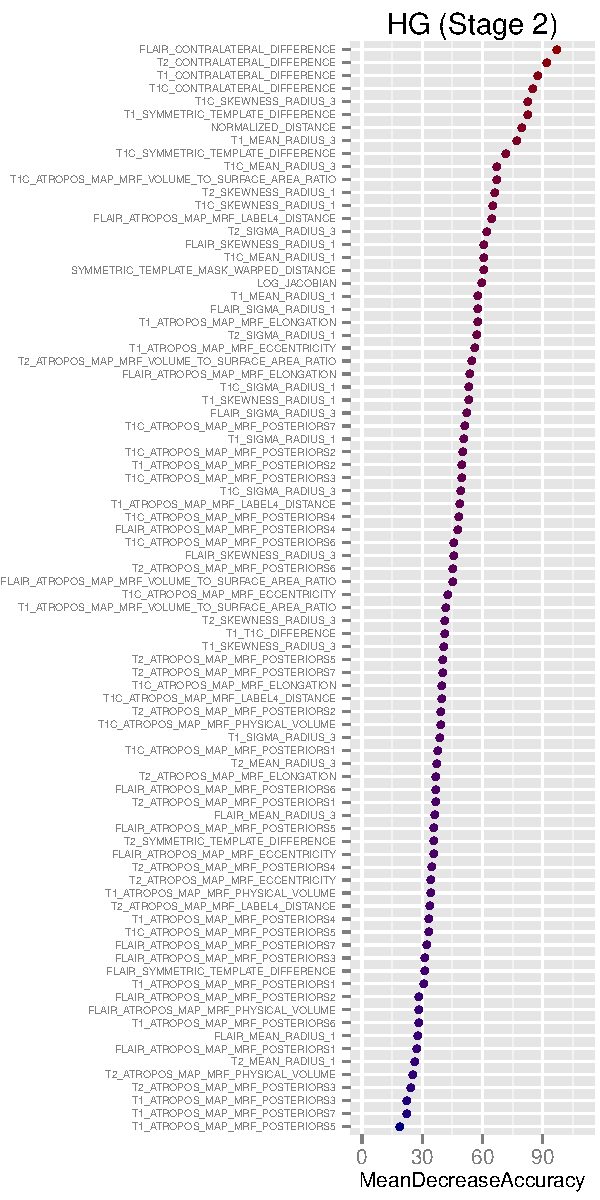
\includegraphics[width=90mm]{Figures/BRATS_HG_MAP_MRF.pdf} \\
  \end{tabular}
  }
  \caption{{\tt MeanDecreaseAccuracy} plots generated from the high-grade glioma
  Stage 1 and Stage 2 RF models.  These plots provide a weighted 
  ranking describing the importance of each feature for predictive accuracy. 
  Features are listed from most to least important.
  }
  \label{fig:hgimportance}
\end{figure*}

\begin{figure*}
  \makebox[\textwidth][c]{
  \begin{tabular}{cc}
  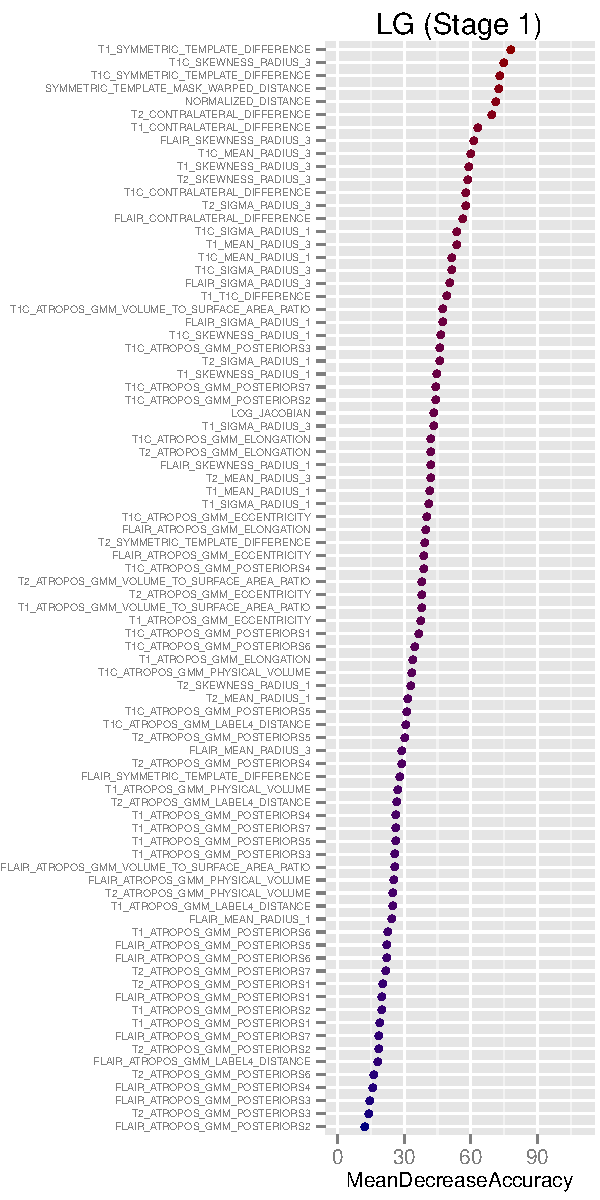
\includegraphics[width=90mm]{Figures/BRATS_LG_GMM.pdf} &
  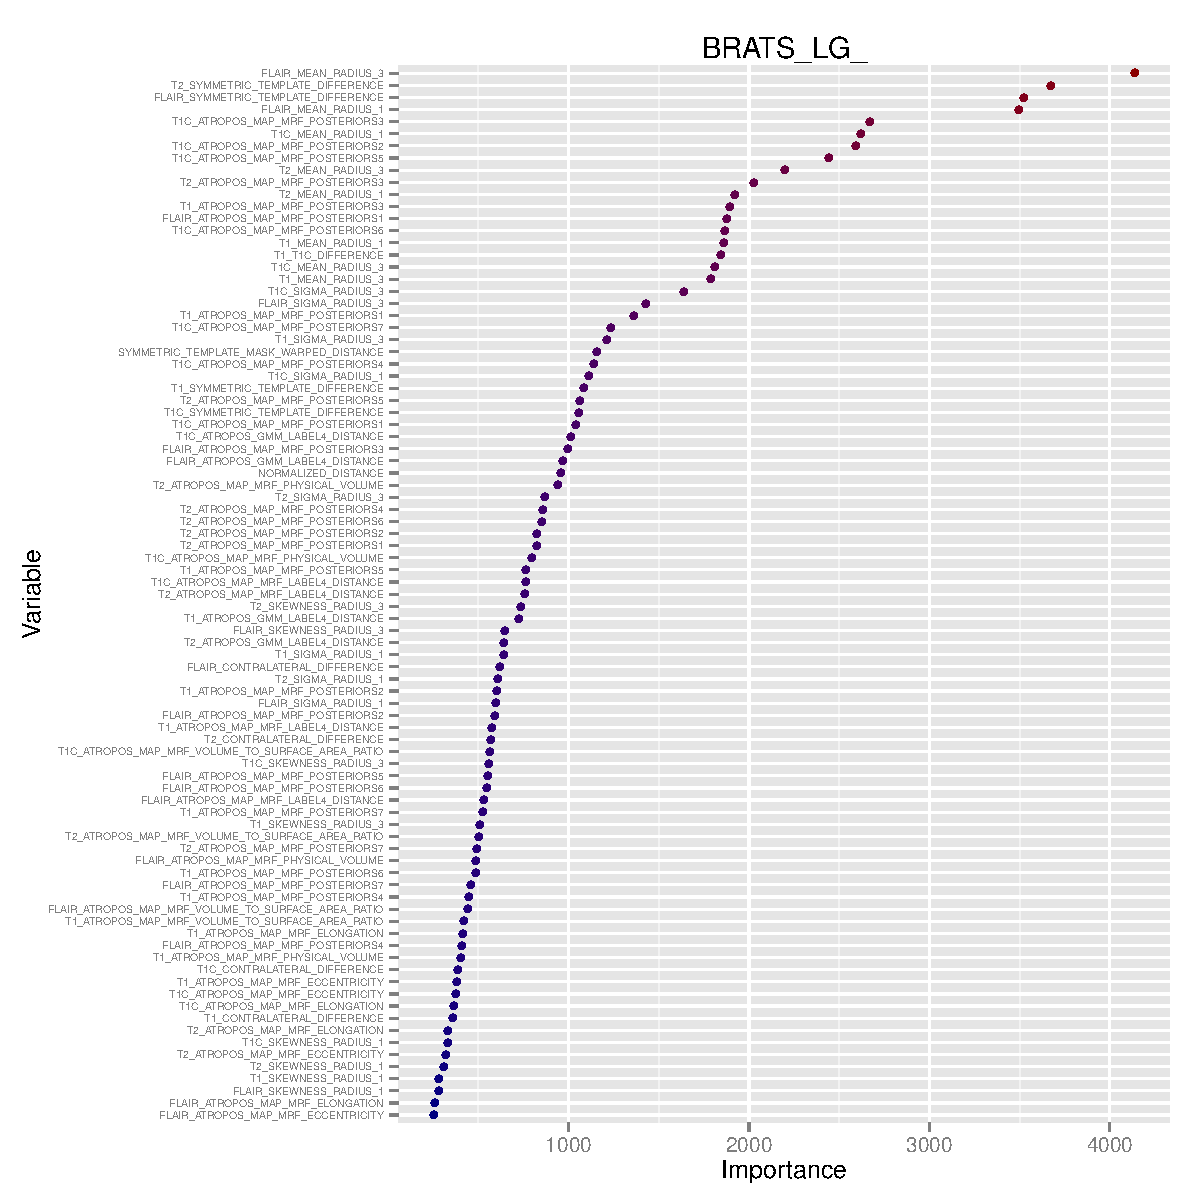
\includegraphics[width=90mm]{Figures/BRATS_LG_MAP_MRF.pdf} \\
  \end{tabular}
  }
  \caption{{\tt MeanDecreaseAccuracy} plots generated from the low-grade glioma
  Stage 1 and Stage 2 RF models.  These plots provide a weighted 
  ranking describing the importance of each feature for predictive accuracy.
  Features are listed from most to least important.
  }
  \label{fig:lgimportance}
\end{figure*}

Immediately apparent from these plots are the importance of certain features.
In general, the features based on the symmetric template are quite
discriminative thus justifying the increased computational 
resources required to generate such features.  For single-threaded processing
on the cluster, creating the feature images for a single subject required 
approximately 2 hours of total processing time of which the template registration 
component took approximately 75\%.  Additionally, the first order 
statistical features also seemed fairly important which is something that
previous work had demonstrated \citep[e.g.,][]{bauer2012,zikic2012}.
There are a number of differences, however, between low-grade and high-grade 
importance outcomes which would also seem to justify the creation of separate
glioma class models.

As described earlier, the MICCAI 2013 BRATS challenge data was provided to the
competitors in three sets.  The Evaluation set was used primarily for training
although an initial ranking was performed for all the competitors to aid in
determining participation in the workshop.  Shortly prior to the actual workshop
date, the Leaderboard data was released to the competitors for posting of results
and subsequent ranking.  Finally, the night before the competition, the Challenge
data was made available and used to produce the final competitor ranking.  In addition
to the Dice overlap measure, additional performance emeasures for producing the rankings 
included the positive predictive value, and sensitivity (all of which can be calculated
using open source tools such as \cite{tustison2009}).  
For all three data sets, we provide these overlap measures and relative competitor 
ranking in Table \ref{table:results}.  Full competition results can be viewed
at {\tt http://www.virtualskeleton.ch}.

\section{Discussion and Conclusions} 

One of the difficulties with the focus of this particular competition 
is the lack of consensus, even clinically, as to tumor type and extent
in the context of medical imaging \citep{cha2005}.  In fact, current 
consensus guidelines from the World Health Organization for brain 
tumor classification are strictly histopathological \citep{louis2007}
which limit clinical application.  Such limitations motivate the
use of medical imaging for treatment planning and outcome analyses 
\citep{cha2005} including more automated methods such as that proposed
in this work.

Although previous research has employed RFs for supervised brain
segmentation, our contribution of concatenated RF model application and use
of symmetric multivariate templates demonstrated good performance 
in the recent MICCAI 2013 Brain Tumor Segmentation challenge/workshop.  
In terms of variable importance, the latter provided several highly 
discriminative features which resulted in the top-performing algorithm 
of the competition.  This confirmed what others have found in that
RFs provide an excellent framework for prediction in certain
medical image analysis problems.  Even with relatively few training
subjects relative to input variables, the RF models
perform well.
In addition, this work highlights the value of  a symmetric multiple
modality template for clinical disorders in which asymmetry is a
hallmark.  Furthermore, our challenge-leading results establish the
value of such templates in multiple modality prediction
tasks in which there is a small training set with an abundance of
multivariate data.

Although these competitions are extremely useful as they provide objective
assessment of algorithmic performance given the prevalence of selection bias
in reporting results in conventional publication venues, even more important
is the availing of the actual algorithmic instantiation (i.e. code) so that
others can more easily build upon and utilize what has proven effective. 
This also provides an opportunity for the users to return
constructive feedback to the authors thereby improving the original offering.  

However, as explained previously, the brain tumor segmentation 
methodology that we have made available is only a small part of the 
larger software package that we have created in \textit{ANTsR}.  Not only does
\textit{ANTsR} significantly facilitate the development of the work discussed,
but it provides an interface to one of the most powerful statistical
packages available in R.  The combination of the well-known ANTs software
package with R provides tremendous potential for future insightful analysis.



%% References with bibTeX database:

%\section*{Acknowledgments}
\clearpage
\section*{References}

\bibliographystyle{elsarticle-harv}
\bibliography{references}
\end{document}
